\documentclass[8pt,aspectratio=1610]{beamer}
\usepackage[utf8]{inputenc}
\usepackage{booktabs}
\usepackage{array}
\usepackage{graphicx}
\usepackage{xcolor}
\usepackage{tikz}
\usetikzlibrary{positioning,arrows.meta,decorations.pathreplacing,calc,shadows}
\usepackage{pgfplots}
\pgfplotsset{compat=1.18}
\usepackage{amsmath}
\usepackage{amssymb}
\usepackage{amsfonts}
\usepackage{algorithm}
\usepackage{algorithmic}

\usetheme{metropolis}
\usecolortheme{wolverine}
\metroset{progressbar=frametitle,block=fill}
\setbeamertemplate{navigation symbols}{}

% Define custom colors complementing the Wolverine theme
\definecolor{maizelight}{RGB}{255, 203, 5}      % Light maize for examples
\definecolor{maizedark}{RGB}{255, 167, 0}       % Darker maize for emphasis
\definecolor{bluelight}{RGB}{0, 39, 76}         % Deep blue for blocks
\definecolor{tealaccent}{RGB}{0, 128, 128}      % Teal for variety
\definecolor{orangeaccent}{RGB}{255, 138, 51}   % Orange complement

% Cross validation specific colors
\definecolor{traincolor}{RGB}{33, 150, 243}     % Blue for training data
\definecolor{validcolor}{RGB}{255, 193, 7}      % Amber for validation data
\definecolor{testcolor}{RGB}{76, 175, 80}       % Green for test data
\definecolor{foldcolor}{RGB}{156, 39, 176}      % Purple for fold highlighting

% Customize block colors
\setbeamercolor{block title}{bg=bluelight,fg=white}
\setbeamercolor{block body}{bg=bluelight!10,fg=black}

% Example blocks in complementary maize
\setbeamercolor{block title example}{bg=maizelight,fg=black}
\setbeamercolor{block body example}{bg=maizelight!15,fg=black}

% Alert blocks in orange accent
\setbeamercolor{block title alerted}{bg=orangeaccent,fg=white}
\setbeamercolor{block body alerted}{bg=orangeaccent!15,fg=black}

% Create custom colored blocks for variety
\newenvironment<>{techblock}[1]{%
  \setbeamercolor{block title}{bg=tealaccent,fg=white}%
  \setbeamercolor{block body}{bg=tealaccent!10,fg=black}%
  \begin{block}#2{#1}}{\end{block}}

\newenvironment<>{tipblock}[1]{%
  \setbeamercolor{block title}{bg=maizedark,fg=black}%
  \setbeamercolor{block body}{bg=maizedark!15,fg=black}%
  \begin{block}#2{#1}}{\end{block}}

% TikZ styles for cross validation diagrams
\tikzset{
    data point/.style={circle, draw, minimum size=0.3cm, inner sep=0pt},
    train data/.style={data point, fill=traincolor!30, draw=traincolor!70},
    valid data/.style={data point, fill=validcolor!30, draw=validcolor!70},
    test data/.style={data point, fill=testcolor!30, draw=testcolor!70},
    fold/.style={rectangle, draw, minimum width=1.5cm, minimum height=0.8cm},
    train fold/.style={fold, fill=traincolor!20, draw=traincolor!70},
    valid fold/.style={fold, fill=validcolor!20, draw=validcolor!70},
    test fold/.style={fold, fill=testcolor!20, draw=testcolor!70},
    fold arrow/.style={->, thick, blue!70},
    cv process/.style={rectangle, rounded corners, draw, fill=gray!10, minimum width=2cm, minimum height=0.6cm}
}

\title{Cross Validation \& Hyperparameter Tuning}
\subtitle{CMSC 173 - Machine Learning}
\author{Course Lecture}
\date{}

\begin{document}

\begin{frame}
\titlepage
\end{frame}

\begin{frame}{Outline}
\tableofcontents
\end{frame}

% ========================================
% Section: Introduction
% ========================================

\section{How to Validate Models?}

\begin{frame}{The Model Validation Problem}
\centering
\textbf{Central Question: How do we assess model performance?}

\vspace{0.5cm}

\begin{columns}[t]
\begin{column}{0.48\textwidth}
\begin{block}{Training Error}
\begin{itemize}
\setlength{\itemsep}{2pt}
\item Error on data used to train the model
\item Always optimistically biased
\item Cannot be used for model selection
\item \textcolor{red}{Misleading indicator}
\end{itemize}
\end{block}
\end{column}

\begin{column}{0.48\textwidth}
\begin{block}{Test Error}
\begin{itemize}
\setlength{\itemsep}{2pt}
\item Error on unseen data
\item True indicator of generalization
\item Should only be used once
\item \textcolor{blue}{Gold standard}
\end{itemize}
\end{block}
\end{column}
\end{columns}

\vspace{0.3cm}

\begin{alertblock}{Problem}
We need to estimate generalization performance \textbf{without} using the test set during model development and hyperparameter tuning.
\end{alertblock}
\end{frame}

\begin{frame}{The Three-Way Data Split}
\centering

\begin{tikzpicture}[scale=1.0, every node/.style={scale=1.0}]
    % Original dataset
    \node[rectangle, draw, fill=gray!20, minimum width=10cm, minimum height=1cm] (dataset) at (0,3) {};
    \node[above=0.1cm of dataset] {\textbf{Original Dataset}};

    % Data split arrows
    \draw[fold arrow, very thick] (-3,2.3) -- (-3,1.7);
    \draw[fold arrow, very thick] (0,2.3) -- (0,1.7);
    \draw[fold arrow, very thick] (3,2.3) -- (3,1.7);

    % Split proportions
    \node at (-3,2) {\scriptsize 60\%};
    \node at (0,2) {\scriptsize 20\%};
    \node at (3,2) {\scriptsize 20\%};

    % Training set
    \node[train fold, minimum width=6cm, minimum height=1cm] (train) at (-3,1) {};
    \node[above=0.1cm of train] {\textbf{Training Set}};
    \node[below=0.1cm of train] {\scriptsize Used to train models};

    % Validation set
    \node[valid fold, minimum width=2cm, minimum height=1cm] (valid) at (0,1) {};
    \node[above=0.1cm of valid] {\textbf{Validation Set}};
    \node[below=0.1cm of valid] {\scriptsize Model selection \& tuning};

    % Test set
    \node[test fold, minimum width=2cm, minimum height=1cm] (test) at (3,1) {};
    \node[above=0.1cm of test] {\textbf{Test Set}};
    \node[below=0.1cm of test] {\scriptsize Final evaluation};

    % Workflow arrows
    \draw[fold arrow, very thick] (train) to[bend left=20] (-1,-0.5);
    \draw[fold arrow, very thick] (valid) -- (0,-0.5);
    \draw[fold arrow, very thick] (test) to[bend right=20] (1,-0.5);

    % Model development process
    \node[cv process, minimum width=3cm] (model) at (0,-1) {\textbf{Model Development}};
    \node[below=0.1cm of model] {\scriptsize Training + Validation};

    % Final evaluation
    \draw[fold arrow, very thick] (model) -- (0,-2.5);
    \node[cv process, fill=testcolor!20, minimum width=2.5cm] (final) at (0,-3) {\textbf{Final Test}};
    \node[below=0.1cm of final] {\scriptsize Unbiased estimate};
\end{tikzpicture}

\vspace{0.3cm}

\begin{alertblock}{Key Insight}
\textbf{Validation set} acts as a proxy for the test set during model development, allowing us to:
\begin{itemize}
\item Compare different models
\item Tune hyperparameters
\item Avoid overfitting to the test set
\end{itemize}
\end{alertblock}
\end{frame}

% ========================================
% Section: Holdout Validation
% ========================================

\section{Holdout Validation}

\begin{frame}{Holdout Validation Method}
\begin{columns}[t]
\begin{column}{0.58\textwidth}
\textbf{Procedure:}
\begin{enumerate}
\setlength{\itemsep}{3pt}
\item Randomly split data into training and validation sets
\item Train model on training set
\item Evaluate on validation set
\item Select best performing model/hyperparameters
\item Final evaluation on held-out test set
\end{enumerate}

\vspace{0.3cm}

\textbf{Common Split Ratios:}
\begin{itemize}
\item 70\% Train, 15\% Validation, 15\% Test
\item 60\% Train, 20\% Validation, 20\% Test
\item 80\% Train, 10\% Validation, 10\% Test
\end{itemize}
\end{column}

\begin{column}{0.38\textwidth}
\begin{block}{Mathematical Formulation}
Given dataset $\mathcal{D} = \{(x_i, y_i)\}_{i=1}^n$:

\begin{align}
\mathcal{D}_{train} &\cup \mathcal{D}_{val} \cup \mathcal{D}_{test} = \mathcal{D} \\
\mathcal{D}_{train} &\cap \mathcal{D}_{val} \cap \mathcal{D}_{test} = \emptyset \\
|\mathcal{D}_{train}| &= \alpha n \\
|\mathcal{D}_{val}| &= \beta n \\
|\mathcal{D}_{test}| &= (1-\alpha-\beta) n
\end{align}

where typically $\alpha \in [0.6, 0.8]$
\end{block}
\end{column}
\end{columns}

\begin{alertblock}{Advantage}
Simple, fast, and provides unbiased estimate when validation set is large enough.
\end{alertblock}
\end{frame}

\begin{frame}{Holdout Validation: Advantages \& Disadvantages}
\begin{columns}[t]
\begin{column}{0.48\textwidth}
\begin{block}{Advantages}
\begin{itemize}
\setlength{\itemsep}{3pt}
\item \textbf{Computational efficiency}: Train model only once
\item \textbf{Simple implementation}: Straightforward to understand and code
\item \textbf{Fast evaluation}: Quick assessment of model performance
\item \textbf{Realistic simulation}: Mimics real-world deployment scenario
\end{itemize}
\end{block}

\begin{block}{When to Use}
\begin{itemize}
\setlength{\itemsep}{2pt}
\item Large datasets (n $>$ 10,000)
\item Computationally expensive models
\item Time-sensitive applications
\end{itemize}
\end{block}
\end{column}

\begin{column}{0.48\textwidth}
\begin{block}{Disadvantages}
\begin{itemize}
\setlength{\itemsep}{3pt}
\item \textbf{High variance}: Performance estimate depends on specific split
\item \textbf{Data inefficiency}: Reduces training data size
\item \textbf{Unreliable for small datasets}: Estimates can be very noisy
\item \textbf{Potential bias}: Unlucky splits can mislead model selection
\end{itemize}
\end{block}

\begin{block}{When NOT to Use}
\begin{itemize}
\setlength{\itemsep}{2pt}
\item Small datasets (n $<$ 1,000)
\item Need for robust performance estimates
\item Critical applications requiring high confidence
\end{itemize}
\end{block}
\end{column}
\end{columns}

\begin{alertblock}{Key Takeaway}
Holdout validation trades robustness for computational efficiency.
\end{alertblock}
\end{frame}

% ========================================
% Section: K-Fold Cross Validation
% ========================================

\section{K-Fold Cross-Validation}

\begin{frame}{K-Fold Cross-Validation Method}
\centering

\begin{tikzpicture}[scale=0.9, every node/.style={scale=0.9}]
    % Title
    \node at (0,4.5) {\textbf{5-Fold Cross-Validation Example}};

    % Original dataset
    \node[rectangle, draw, fill=gray!20, minimum width=10cm, minimum height=0.6cm] (dataset) at (0,4) {};
    \node[left=0.2cm of dataset] {\scriptsize Original Data:};

    % Fold 1
    \node[valid fold, minimum width=2cm, minimum height=0.6cm] (f1v) at (-4,3) {};
    \node[train fold, minimum width=8cm, minimum height=0.6cm] (f1t) at (0,3) {};
    \node[left=0.2cm of f1v] {\scriptsize Fold 1:};
    \node[below=0.05cm of f1v] {\tiny Valid};
    \node[below=0.05cm of f1t] {\tiny Train};

    % Fold 2
    \node[train fold, minimum width=2cm, minimum height=0.6cm] (f2t1) at (-4,2.2) {};
    \node[valid fold, minimum width=2cm, minimum height=0.6cm] (f2v) at (-2,2.2) {};
    \node[train fold, minimum width=6cm, minimum height=0.6cm] (f2t2) at (1,2.2) {};
    \node[left=0.2cm of f2t1] {\scriptsize Fold 2:};
    \node[below=0.05cm of f2v] {\tiny Valid};

    % Fold 3
    \node[train fold, minimum width=4cm, minimum height=0.6cm] (f3t1) at (-3,1.4) {};
    \node[valid fold, minimum width=2cm, minimum height=0.6cm] (f3v) at (0,1.4) {};
    \node[train fold, minimum width=4cm, minimum height=0.6cm] (f3t2) at (3,1.4) {};
    \node[left=0.2cm of f3t1] {\scriptsize Fold 3:};
    \node[below=0.05cm of f3v] {\tiny Valid};

    % Fold 4
    \node[train fold, minimum width=6cm, minimum height=0.6cm] (f4t1) at (-2,0.6) {};
    \node[valid fold, minimum width=2cm, minimum height=0.6cm] (f4v) at (2,0.6) {};
    \node[train fold, minimum width=2cm, minimum height=0.6cm] (f4t2) at (4,0.6) {};
    \node[left=0.2cm of f4t1] {\scriptsize Fold 4:};
    \node[below=0.05cm of f4v] {\tiny Valid};

    % Fold 5
    \node[train fold, minimum width=8cm, minimum height=0.6cm] (f5t) at (-1,-0.2) {};
    \node[valid fold, minimum width=2cm, minimum height=0.6cm] (f5v) at (4,-0.2) {};
    \node[left=0.2cm of f5t] {\scriptsize Fold 5:};
    \node[below=0.05cm of f5v] {\tiny Valid};

    % Results aggregation
    \draw[fold arrow, very thick] (-2,-0.8) -- (-2,-1.5);
    \draw[fold arrow, very thick] (0,-0.8) -- (0,-1.5);
    \draw[fold arrow, very thick] (2,-0.8) -- (2,-1.5);

    \node[cv process, minimum width=6cm] (aggregate) at (0,-2) {\textbf{Average Results}};
    \node[below=0.1cm of aggregate] {\scriptsize $CV_{score} = \frac{1}{k}\sum_{i=1}^{k} Score_i$};
\end{tikzpicture}

\vspace{0.3cm}

\begin{alertblock}{Core Idea}
Use \textbf{all data} for both training and validation by systematically rotating which portion serves as the validation set.
\end{alertblock}
\end{frame}

\begin{frame}{K-Fold Cross-Validation: Mathematical Formulation}
\textbf{Algorithm:}
\begin{enumerate}
\setlength{\itemsep}{3pt}
\item Partition dataset $\mathcal{D}$ into $k$ equal-sized folds: $\mathcal{D} = \mathcal{D}_1 \cup \mathcal{D}_2 \cup \cdots \cup \mathcal{D}_k$
\item For each fold $i = 1, \ldots, k$:
\begin{itemize}
\item Training set: $\mathcal{D}_{train}^{(i)} = \mathcal{D} \setminus \mathcal{D}_i$
\item Validation set: $\mathcal{D}_{val}^{(i)} = \mathcal{D}_i$
\item Train model $f^{(i)}$ on $\mathcal{D}_{train}^{(i)}$
\item Compute validation error: $E^{(i)} = L(f^{(i)}, \mathcal{D}_{val}^{(i)})$
\end{itemize}
\item Estimate generalization error: $\hat{E}_{CV} = \frac{1}{k}\sum_{i=1}^k E^{(i)}$
\end{enumerate}

\vspace{0.3cm}

\begin{columns}[t]
\begin{column}{0.48\textwidth}
\begin{block}{Error Estimation}
$$\hat{E}_{CV} = \frac{1}{k}\sum_{i=1}^k L(f^{(i)}, \mathcal{D}_i)$$

$$\text{Var}(\hat{E}_{CV}) = \frac{1}{k^2}\sum_{i=1}^k \text{Var}(E^{(i)})$$
\end{block}
\end{column}

\begin{column}{0.48\textwidth}
\begin{block}{Standard Error}
$$SE(\hat{E}_{CV}) = \sqrt{\frac{1}{k}\sum_{i=1}^k \left(E^{(i)} - \hat{E}_{CV}\right)^2}$$

Confidence interval: $\hat{E}_{CV} \pm 1.96 \cdot SE$
\end{block}
\end{column}
\end{columns}
\end{frame}

\begin{frame}{Choice of k in K-Fold Cross-Validation}
\begin{columns}[t]
\begin{column}{0.58\textwidth}
\textbf{Common Values:}
\begin{itemize}
\setlength{\itemsep}{4pt}
\item \textbf{k = 5}: Good balance, widely used
\item \textbf{k = 10}: Most popular, good bias-variance tradeoff
\item \textbf{k = n (LOOCV)}: Lowest bias, highest variance
\end{itemize}

\vspace{0.3cm}

\textbf{Bias-Variance Tradeoff:}
\begin{align}
\text{Bias} &\propto \frac{k-1}{k} \text{ (decreases with k)} \\
\text{Variance} &\propto \text{correlation between folds} \\
\text{Computation} &\propto k \text{ (increases with k)}
\end{align}
\end{column}

\begin{column}{0.38\textwidth}
\begin{block}{Choosing k}
\textbf{Small k (k = 3-5):}
\begin{itemize}
\item Higher bias
\item Lower variance
\item Less computation
\item Good for large datasets
\end{itemize}

\vspace{0.2cm}

\textbf{Large k (k = 10-20):}
\begin{itemize}
\item Lower bias
\item Higher variance
\item More computation
\item Good for small datasets
\end{itemize}
\end{block}
\end{column}
\end{columns}

\begin{alertblock}{Recommendation}
Use \textbf{k = 10} as default choice. It provides good bias-variance tradeoff for most practical scenarios.
\end{alertblock}
\end{frame}

\begin{frame}{K-Fold vs Holdout: Performance Comparison}
\centering
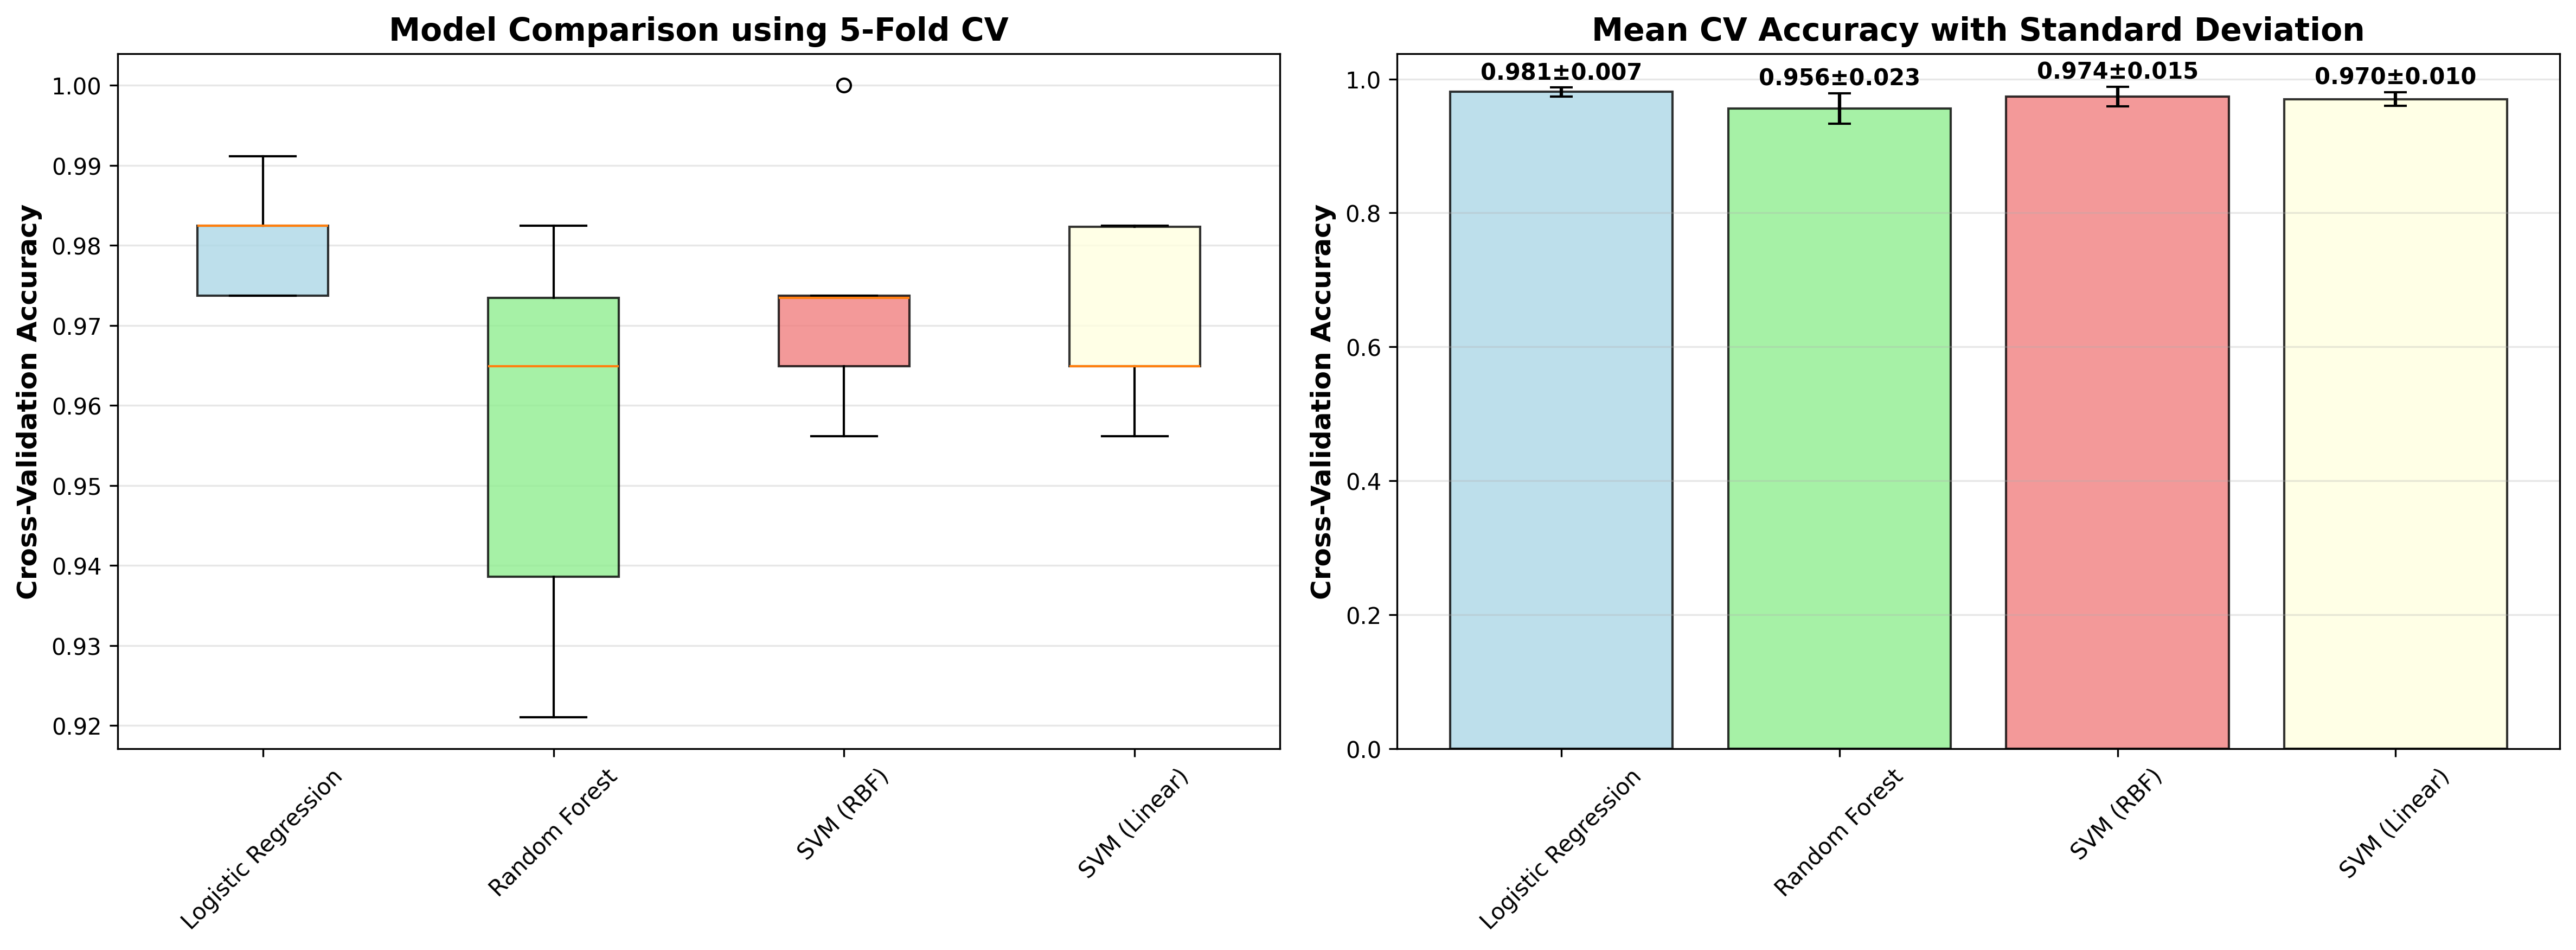
\includegraphics[width=0.9\textwidth]{../figures/model_comparison_cv.png}

\vspace{0.3cm}

\begin{alertblock}{Key Observation}
K-fold cross-validation provides more robust and reliable performance estimates, especially important for model comparison and selection.
\end{alertblock}
\end{frame}

% ========================================
% Section: Other Validation Methods
% ========================================

\section{Other Variants}

\begin{frame}{Leave-One-Out Cross-Validation (LOOCV)}
\centering
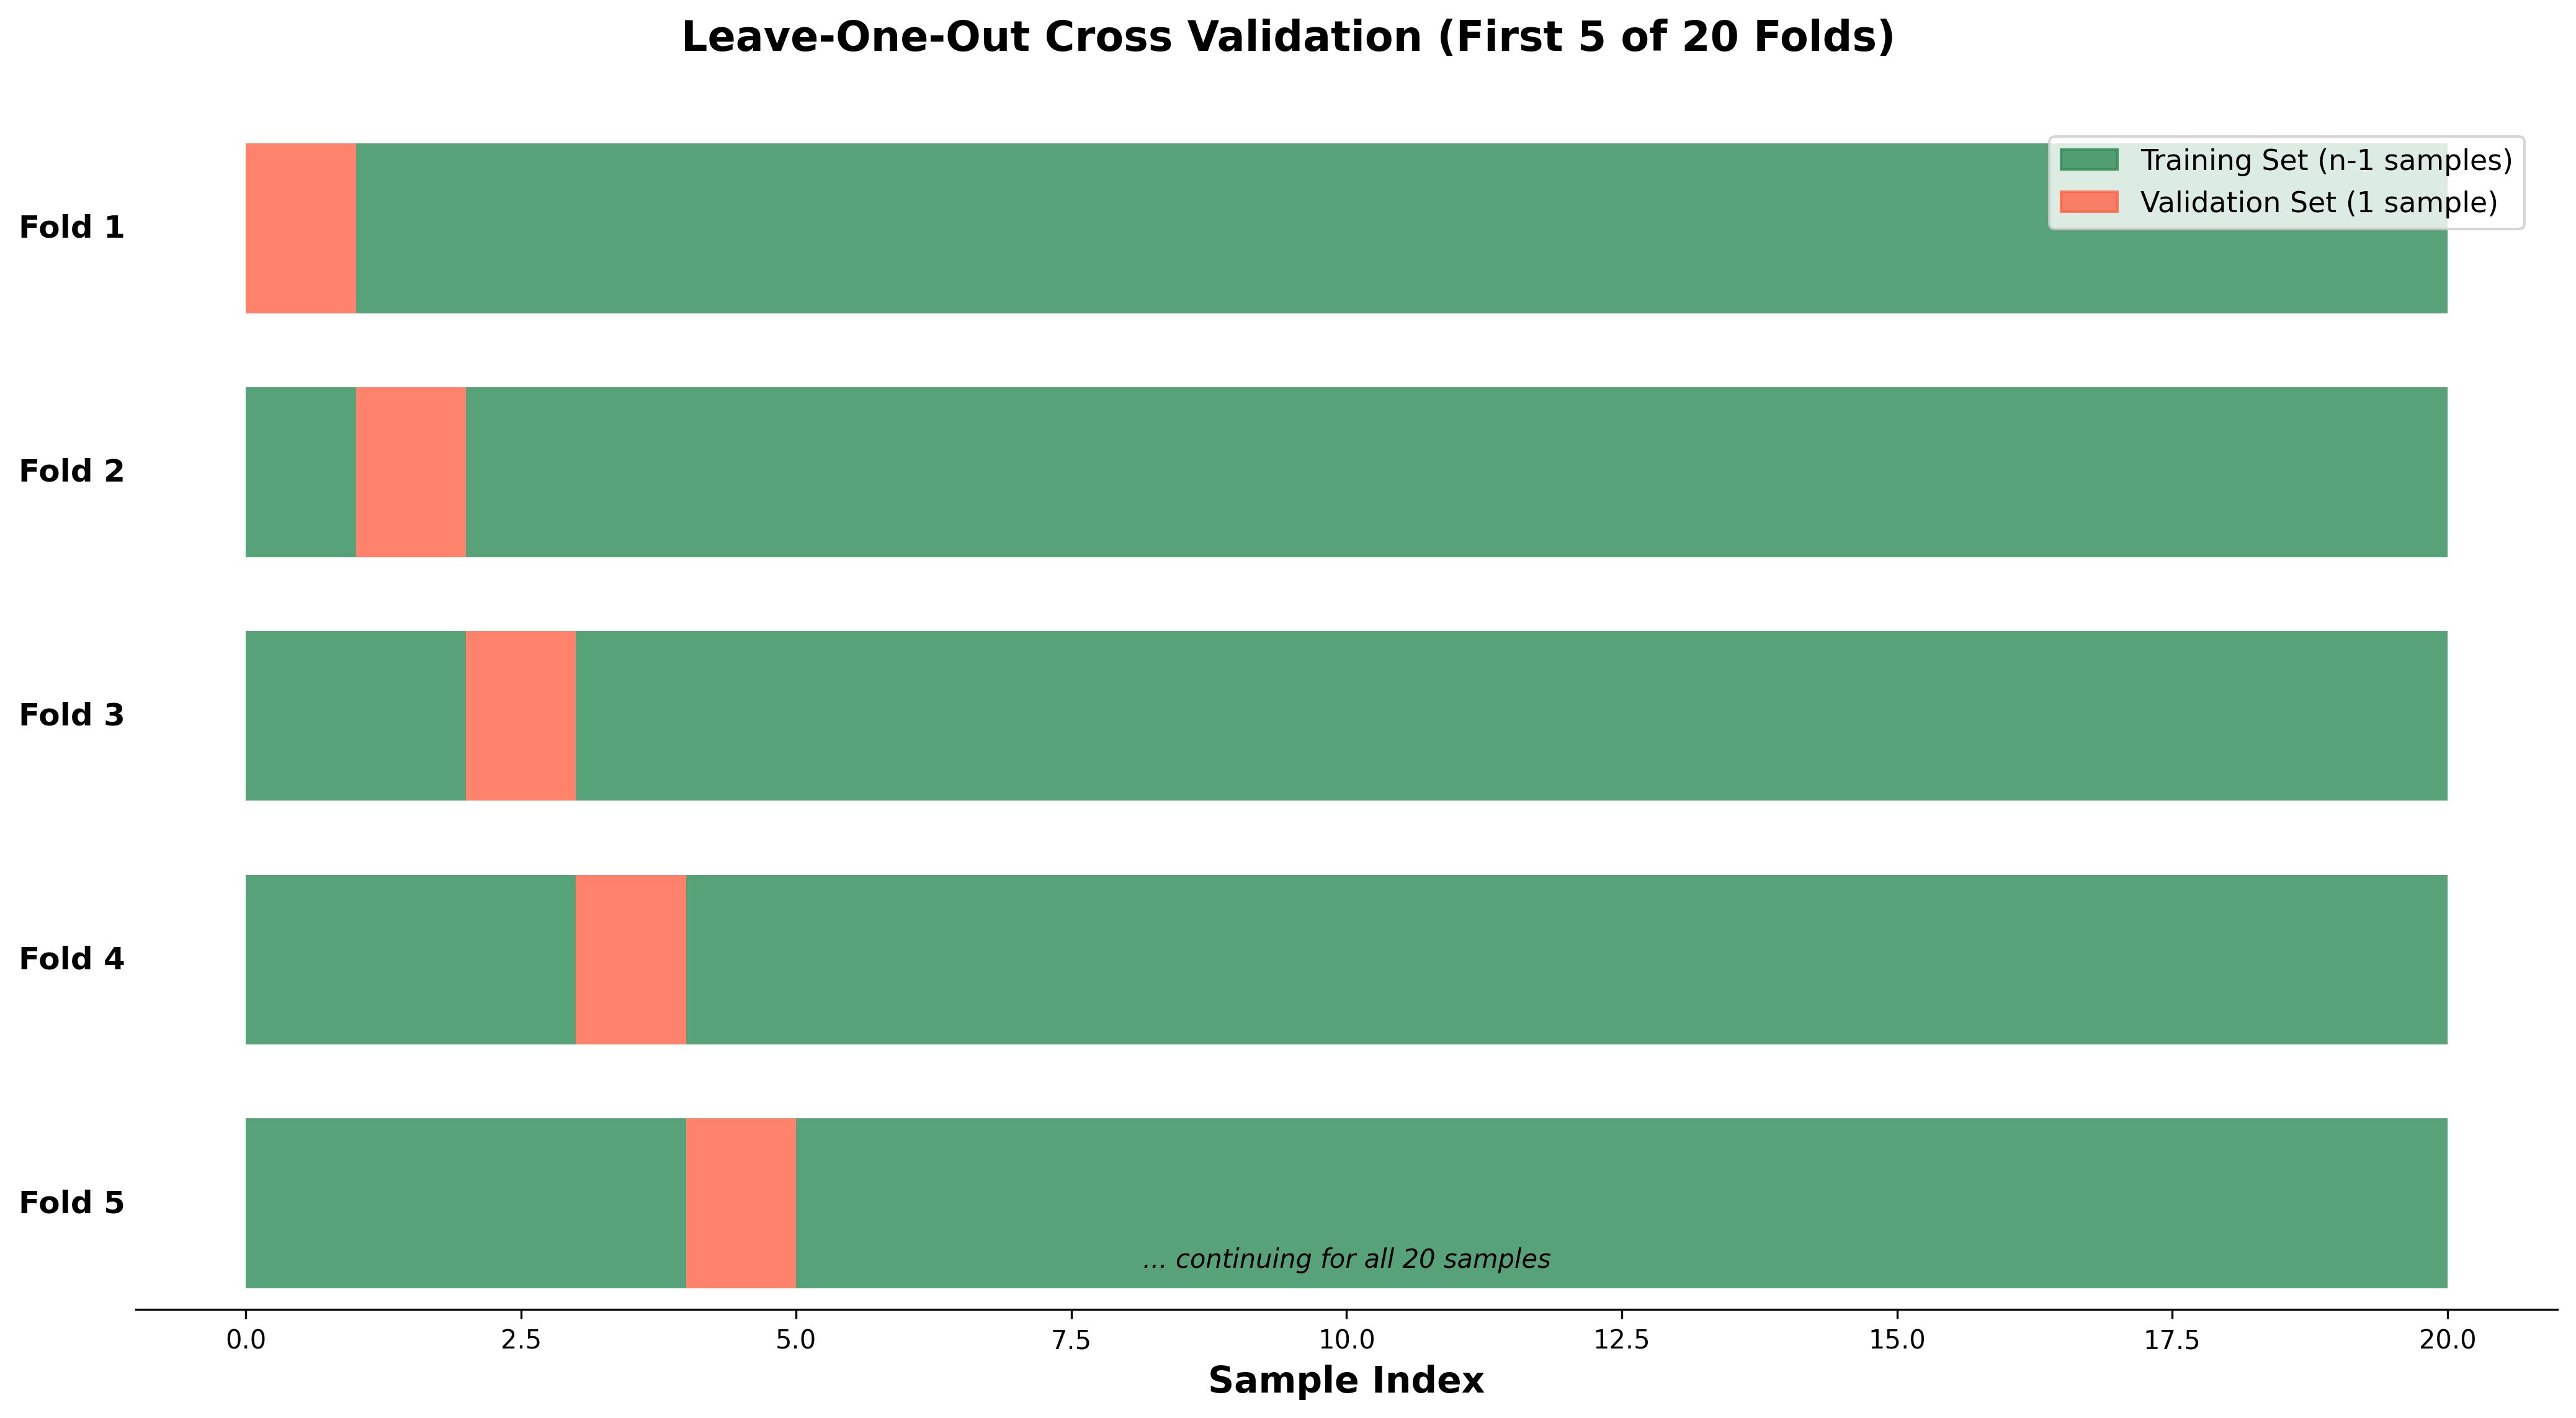
\includegraphics[width=0.75\textwidth]{../figures/loocv_validation.png}

\vspace{0.3cm}

\begin{columns}[t]
\begin{column}{0.48\textwidth}
\begin{block}{Mathematical Formulation}
LOOCV is k-fold CV with $k = n$:
$$\hat{E}_{LOOCV} = \frac{1}{n}\sum_{i=1}^n L(f^{(-i)}, (x_i, y_i))$$

where $f^{(-i)}$ is trained on all data except $(x_i, y_i)$.
\end{block}
\end{column}

\begin{column}{0.48\textwidth}
\begin{block}{Properties}
\begin{itemize}
\setlength{\itemsep}{3pt}
\item \textbf{Bias}: Nearly unbiased (uses n-1 samples)
\item \textbf{Variance}: High (high correlation between folds)
\item \textbf{Computation}: Expensive (n model fits)
\item \textbf{Deterministic}: No randomness in splits
\end{itemize}
\end{block}
\end{column}
\end{columns}

\begin{alertblock}{When to Use LOOCV}
Small datasets where every sample is precious, and computational cost is acceptable.
\end{alertblock}
\end{frame}

\begin{frame}{Stratified K-Fold Cross-Validation}
\centering
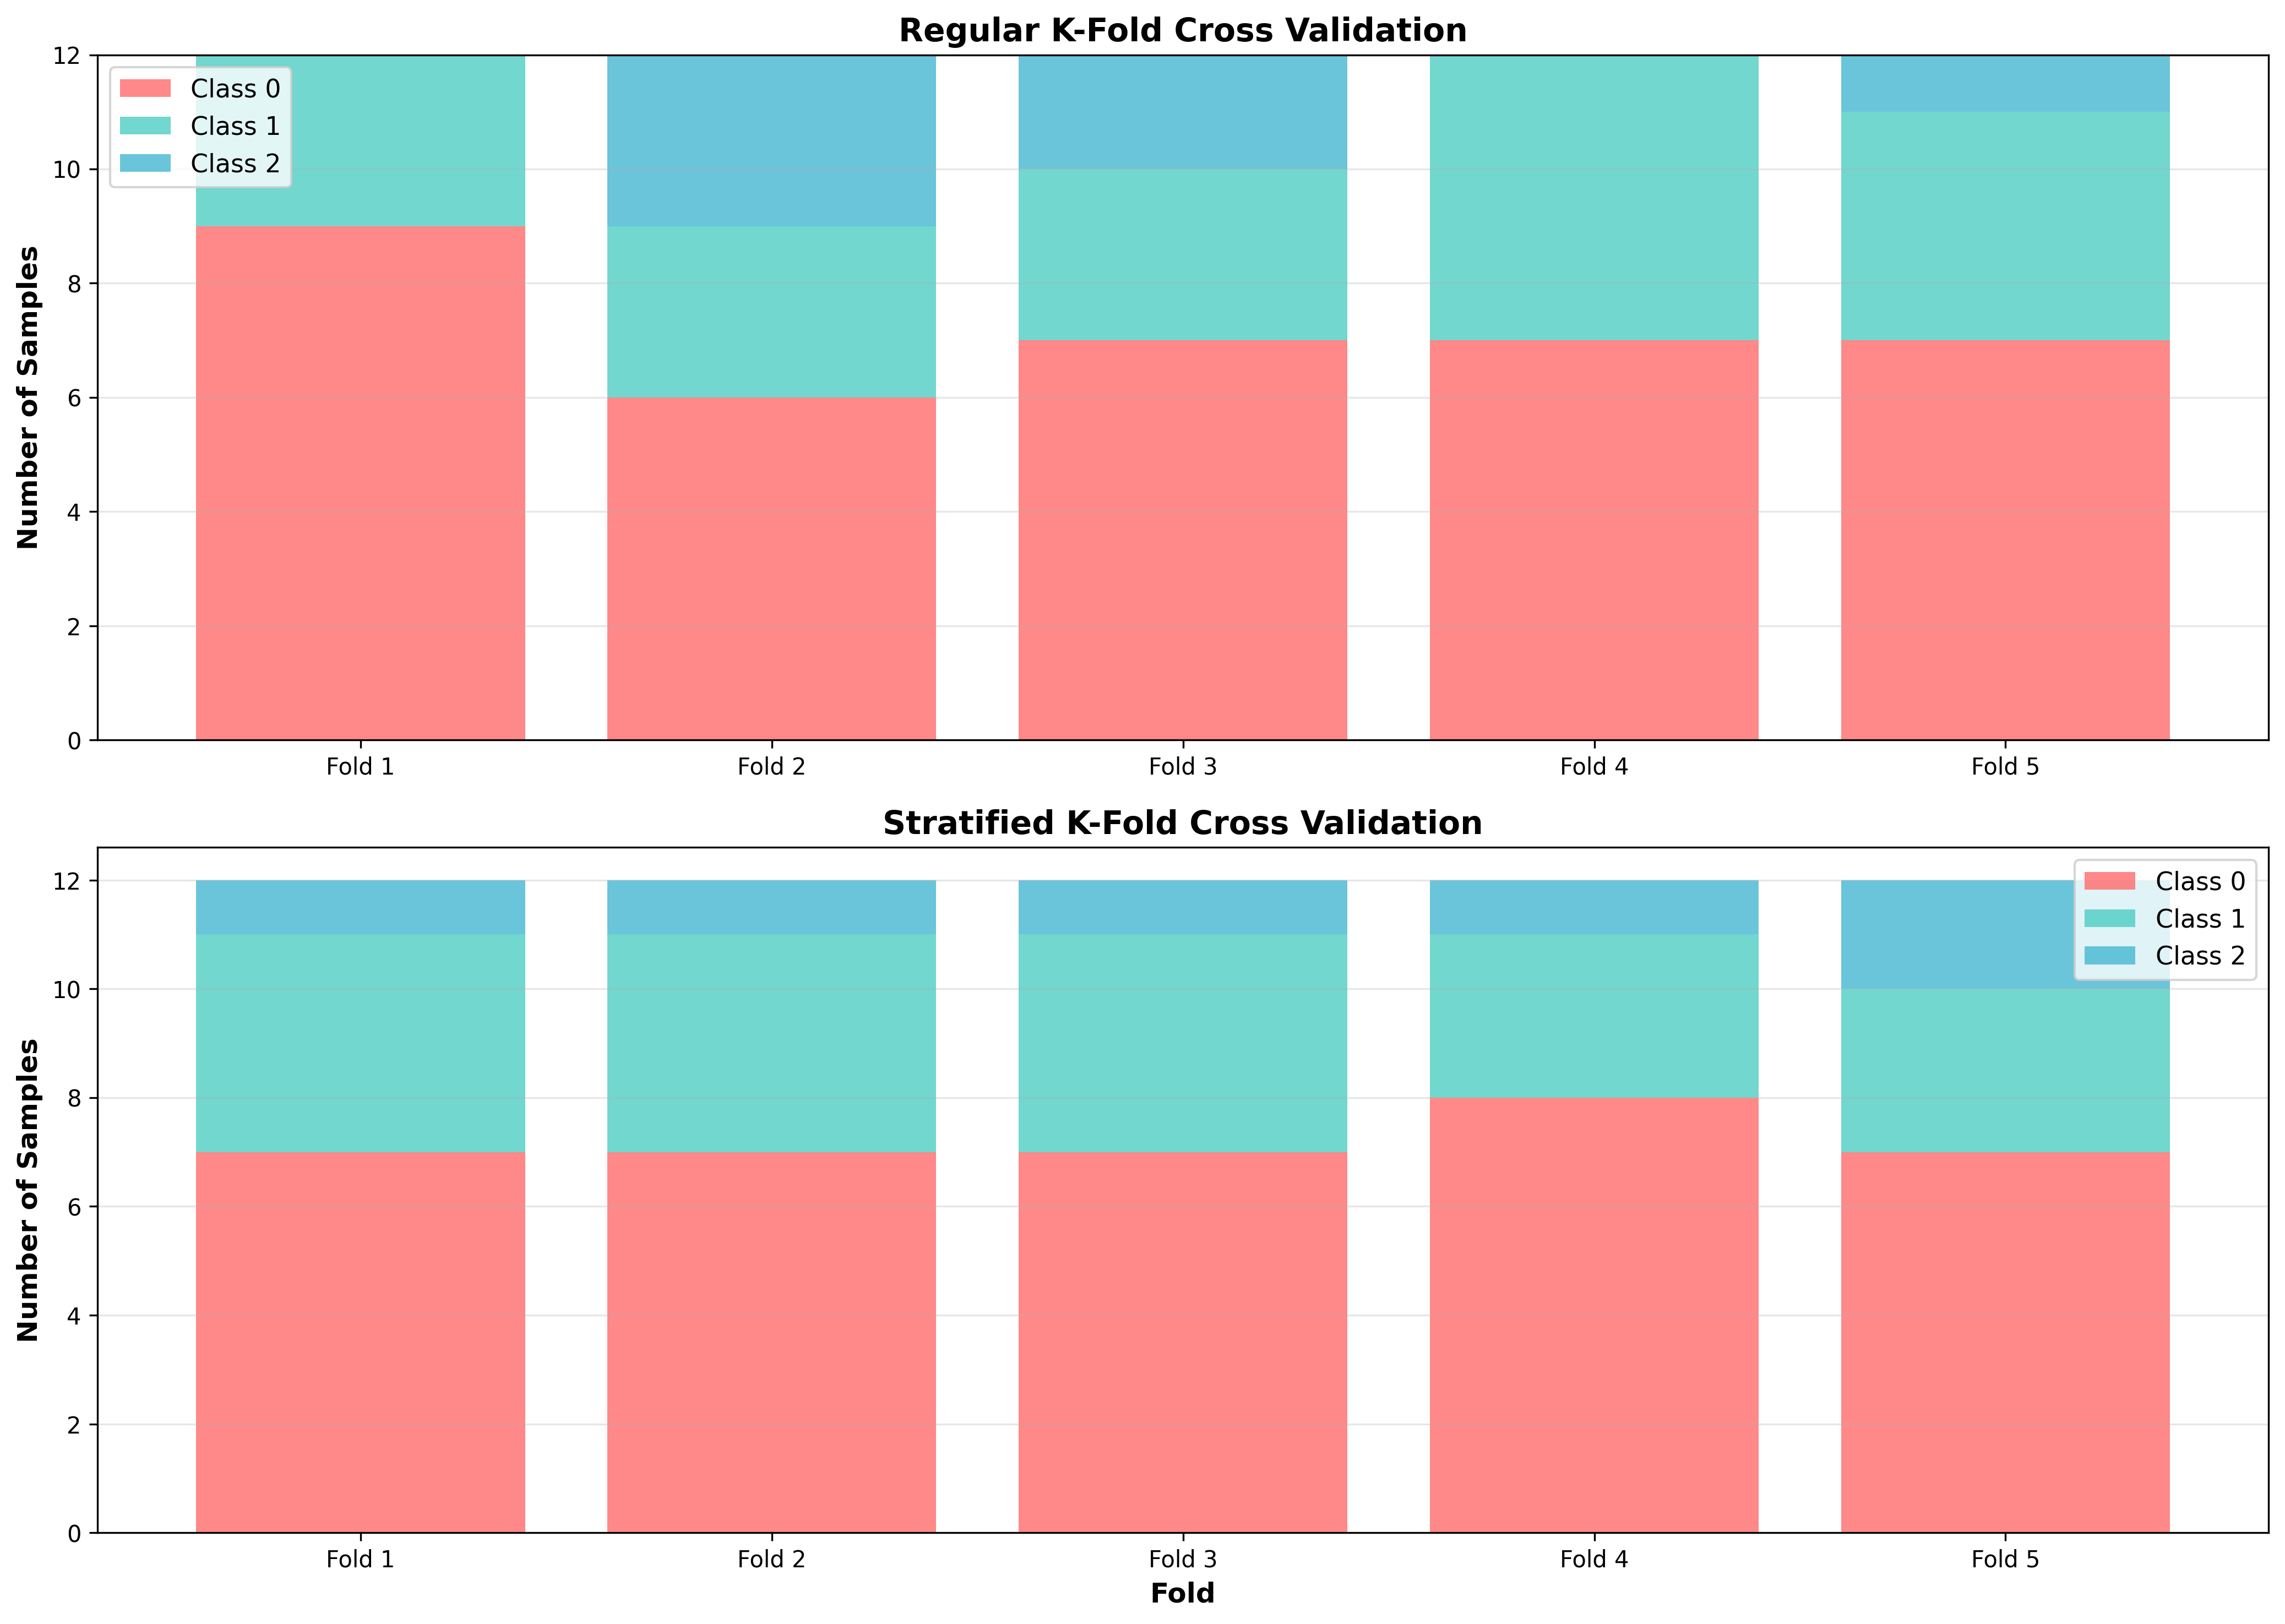
\includegraphics[width=0.75\textwidth]{../figures/stratified_kfold_comparison.png}

\vspace{0.3cm}

\begin{alertblock}{Key Advantage}
Maintains class distribution across folds, crucial for:
\begin{itemize}
\item \textbf{Imbalanced datasets}: Ensures each fold has representatives from all classes
\item \textbf{Small datasets}: Prevents folds with missing classes
\item \textbf{Multiclass problems}: Maintains proportional representation
\end{itemize}
\end{alertblock}
\end{frame}

\begin{frame}{Specialized Cross-Validation Methods}
\begin{columns}[t]
\begin{column}{0.48\textwidth}
\begin{block}{Time Series Cross-Validation}
\textbf{Problem:} Standard CV violates temporal order

\textbf{Solution:} Forward chaining
\begin{itemize}
\item Fold 1: Train[1:100], Test[101:150]
\item Fold 2: Train[1:150], Test[151:200]
\item Fold 3: Train[1:200], Test[201:250]
\end{itemize}

\textbf{Preserves:} Temporal dependencies
\end{block}

\begin{block}{Group K-Fold}
\textbf{Problem:} Data points are grouped (e.g., patients, images from same source)

\textbf{Solution:} Ensure entire groups stay together in splits

\textbf{Prevents:} Data leakage between folds
\end{block}
\end{column}

\begin{column}{0.48\textwidth}
\begin{block}{Monte Carlo Cross-Validation}
\textbf{Method:} Random sampling approach
\begin{itemize}
\item Randomly split data multiple times
\item Average performance across all splits
\item More flexible than k-fold
\end{itemize}

\textbf{Advantage:} Can control train/validation ratio
\end{block}

\begin{block}{Nested Cross-Validation}
\textbf{Purpose:} Unbiased model selection + evaluation

\textbf{Structure:}
\begin{itemize}
\item Outer loop: Performance estimation
\item Inner loop: Hyperparameter tuning
\end{itemize}

\textbf{Result:} True generalization estimate
\end{block}
\end{column}
\end{columns}

\begin{alertblock}{Guideline}
Choose validation method based on data characteristics and problem constraints.
\end{alertblock}
\end{frame}

% ========================================
% Section: Hyperparameter Search Methods
% ========================================

\section{Hyper-parameter Search Methods}

\begin{frame}{The Hyperparameter Optimization Problem}
\begin{columns}[t]
\begin{column}{0.55\textwidth}
\textbf{Goal:} Find optimal hyperparameters $\lambda^*$

\begin{align}
\lambda^* &= \arg\min_{\lambda \in \Lambda} \hat{E}_{CV}(\lambda) \\
\hat{E}_{CV}(\lambda) &= \frac{1}{k}\sum_{i=1}^k L(f_\lambda^{(i)}, \mathcal{D}_i)
\end{align}

where:
\begin{itemize}
\item $\lambda$: hyperparameter vector
\item $\Lambda$: search space
\item $f_\lambda^{(i)}$: model trained with $\lambda$ on fold $i$
\end{itemize}
\end{column}

\begin{column}{0.41\textwidth}
\begin{exampleblock}{Examples}
\textbf{SVM:} $\lambda = (C, \gamma)$
$$\Lambda = [10^{-3}, 10^3] \times [10^{-6}, 10^1]$$

\textbf{Random Forest:}
$$\lambda = (n_{est}, \text{depth}, \text{features})$$

\textbf{Neural Network:}
$$\lambda = (lr, \text{batch}, \text{layers}, \text{dropout})$$
\end{exampleblock}
\end{column}
\end{columns}

\vspace{0.3cm}

\begin{alertblock}{Challenge}
Hyperparameter spaces are often high-dimensional, mixed-type, and expensive to evaluate.
\end{alertblock}
\end{frame}

% ========================================
% Section: Grid Search
% ========================================

\section{Grid Search}

\begin{frame}{Grid Search Method}
\centering
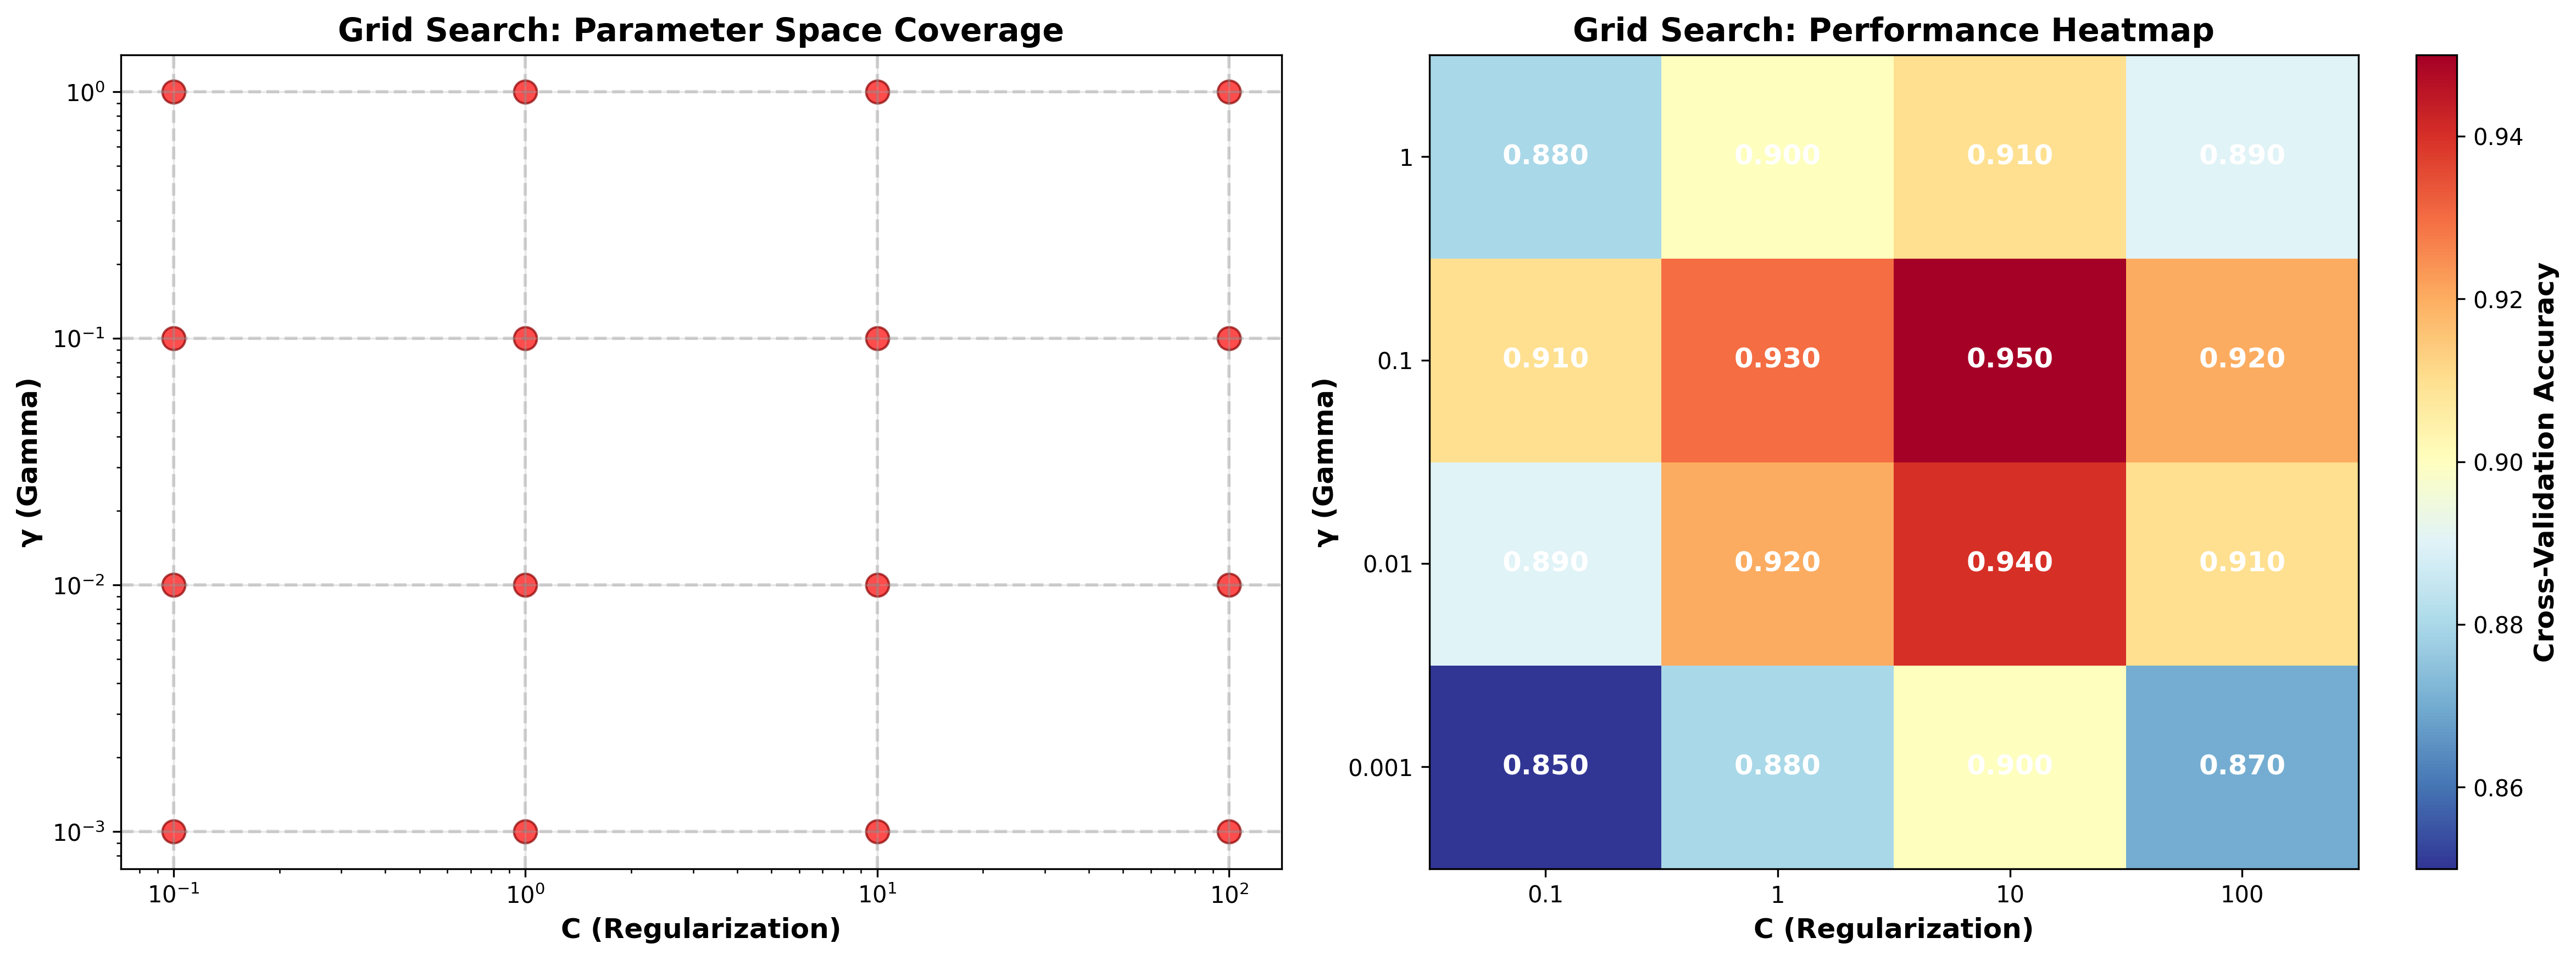
\includegraphics[width=0.9\textwidth]{../figures/grid_search_visualization.png}

\vspace{0.3cm}

\begin{alertblock}{Core Principle}
\textbf{Exhaustive search} over a discrete grid of hyperparameter combinations.
\end{alertblock}
\end{frame}

\begin{frame}{Grid Search: Mathematical Formulation}
\textbf{Algorithm:}
\begin{enumerate}
\setlength{\itemsep}{3pt}
\item Define search grid: $\Lambda_{grid} = \{\lambda_1, \lambda_2, \ldots, \lambda_m\}$
\item For each $\lambda_j \in \Lambda_{grid}$:
\begin{itemize}
\item Compute $\hat{E}_{CV}(\lambda_j)$ using k-fold cross-validation
\item Store result: $(\lambda_j, \hat{E}_{CV}(\lambda_j))$
\end{itemize}
\item Return: $\lambda^* = \arg\min_{\lambda_j} \hat{E}_{CV}(\lambda_j)$
\end{enumerate}

\vspace{0.3cm}

\begin{columns}[t]
\begin{column}{0.48\textwidth}
\begin{block}{Grid Construction}
For parameter $\lambda_i$ with range $[a_i, b_i]$:

\textbf{Linear spacing:}
$$\lambda_i^{(j)} = a_i + \frac{j-1}{n_i-1}(b_i - a_i)$$

\textbf{Log spacing (preferred for scale-invariant parameters):}
$$\lambda_i^{(j)} = a_i \cdot \left(\frac{b_i}{a_i}\right)^{\frac{j-1}{n_i-1}}$$
\end{block}
\end{column}

\begin{column}{0.48\textwidth}
\begin{block}{Computational Complexity}
Total evaluations: $\prod_{i=1}^p n_i$

With k-fold CV:
$$\text{Total cost} = k \cdot \prod_{i=1}^p n_i \cdot C_{train}$$

where:
\begin{itemize}
\item $p$: number of hyperparameters
\item $n_i$: grid points for parameter $i$
\item $C_{train}$: cost of training one model
\end{itemize}
\end{block}
\end{column}
\end{columns}
\end{frame}

\begin{frame}{Grid Search: Advantages \& Disadvantages}
\begin{columns}[t]
\begin{column}{0.48\textwidth}
\begin{block}{Advantages}
\begin{itemize}
\setlength{\itemsep}{3pt}
\item \textbf{Exhaustive}: Guarantees finding the best combination on the grid
\item \textbf{Parallel}: Evaluations are independent
\item \textbf{Reproducible}: Deterministic results
\item \textbf{Simple}: Easy to implement and understand
\item \textbf{Complete coverage}: Systematic exploration
\end{itemize}
\end{block}

\begin{block}{Best Practices}
\begin{itemize}
\setlength{\itemsep}{2pt}
\item Use log-uniform grids for scale parameters (C, $\gamma$, learning rate)
\item Start with coarse grid, refine around promising regions
\item Use domain knowledge for range selection
\end{itemize}
\end{block}
\end{column}

\begin{column}{0.48\textwidth}
\begin{block}{Disadvantages}
\begin{itemize}
\setlength{\itemsep}{3pt}
\item \textbf{Curse of dimensionality}: Exponential growth with parameters
\item \textbf{Computational cost}: Can be prohibitively expensive
\item \textbf{Grid limitations}: Optimal values might lie between grid points
\item \textbf{Uniform sampling}: Wastes effort in unpromising regions
\item \textbf{Manual tuning}: Requires careful grid design
\end{itemize}
\end{block}

\begin{block}{When NOT to Use}
\begin{itemize}
\setlength{\itemsep}{2pt}
\item High-dimensional hyperparameter spaces ($p > 4$)
\item Expensive model training ($C_{train}$ very large)
\item Continuous optimization required
\end{itemize}
\end{block}
\end{column}
\end{columns}

\begin{alertblock}{Rule of Thumb}
Grid search is practical for $\leq$ 3-4 hyperparameters with reasonable computational budget.
\end{alertblock}
\end{frame}

% ========================================
% Section: Random Search
% ========================================

\section{Random Search}

\begin{frame}{Random Search vs Grid Search}
\centering
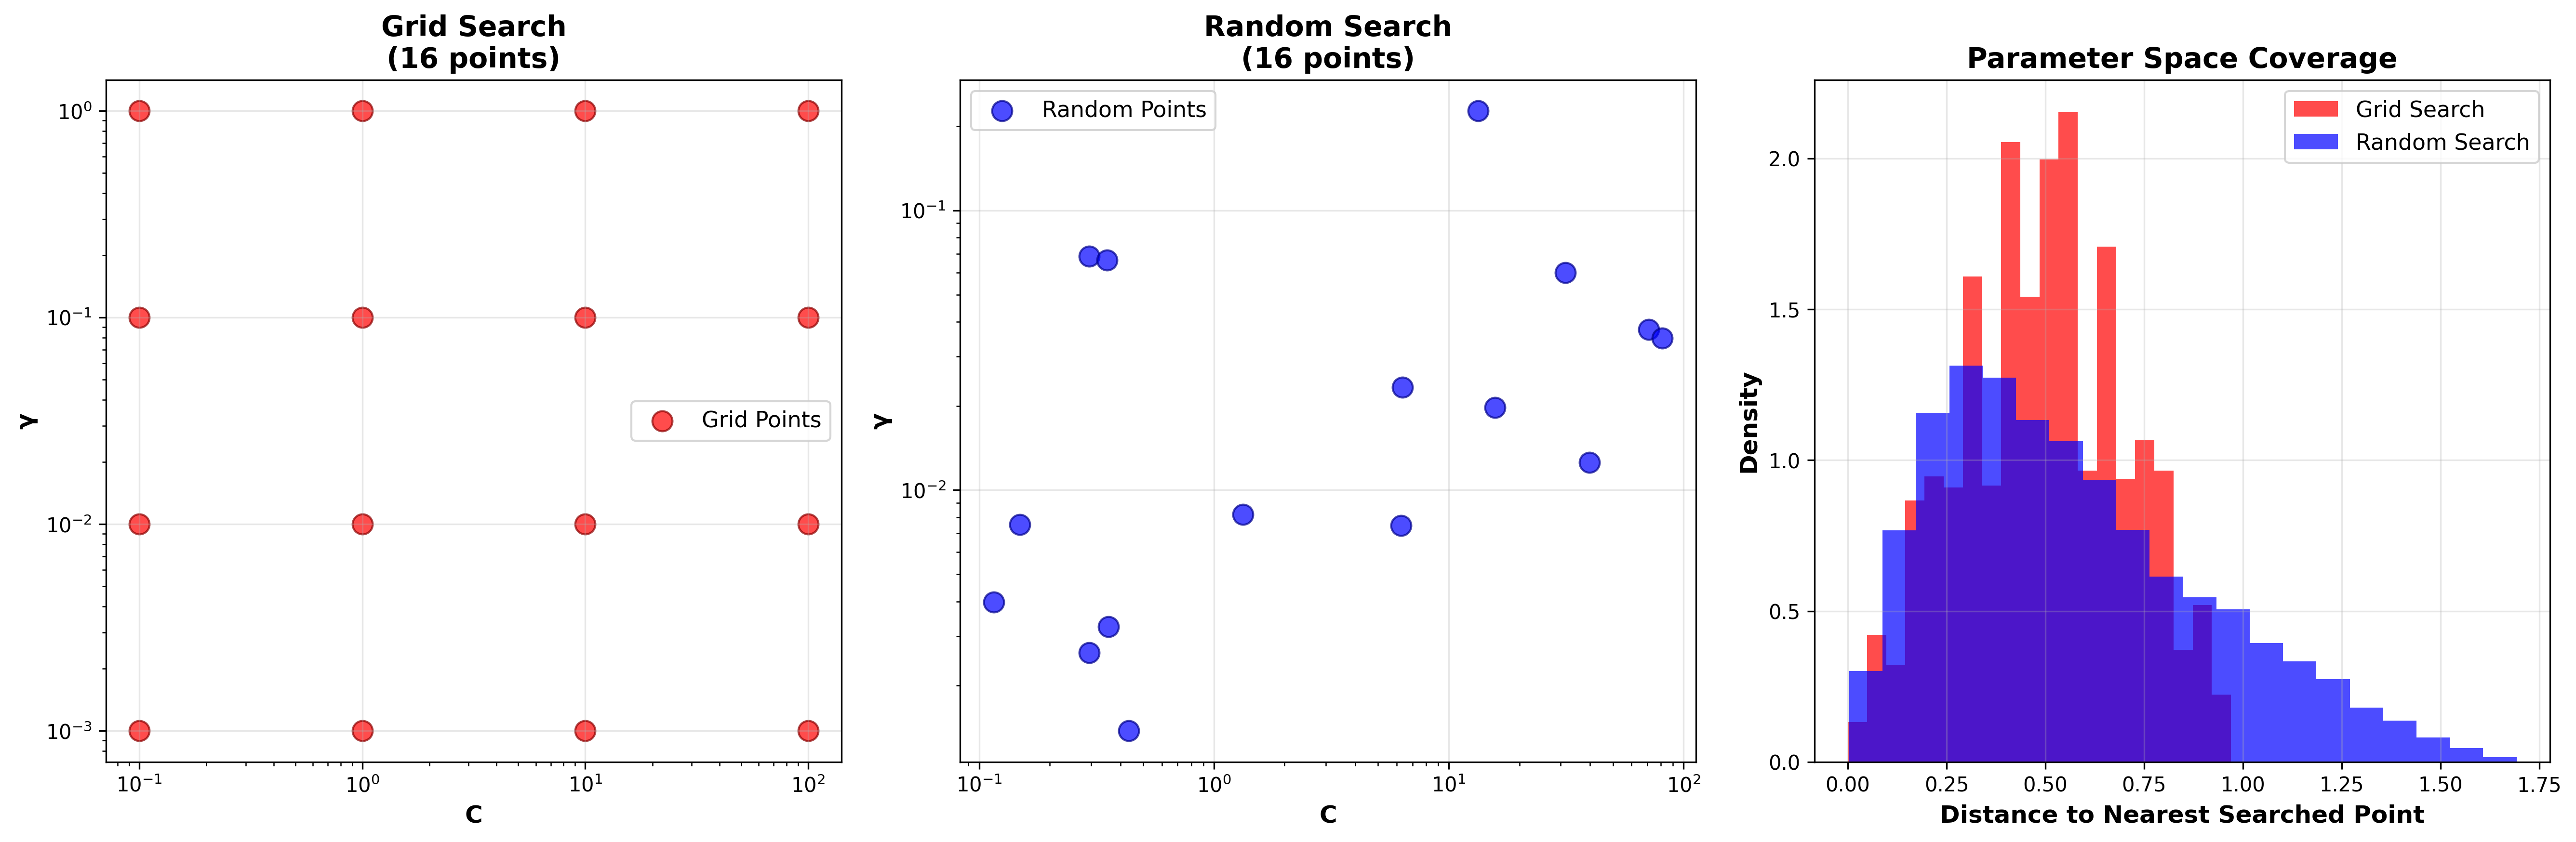
\includegraphics[width=0.9\textwidth]{../figures/random_vs_grid_search.png}

\vspace{0.3cm}

\begin{alertblock}{Key Insight}
Random search often finds better solutions than grid search with the same computational budget, especially in high dimensions.
\end{alertblock}
\end{frame}

\begin{frame}{Random Search: Method \& Theory}
\textbf{Algorithm:}
\begin{enumerate}
\setlength{\itemsep}{3pt}
\item Define parameter distributions: $\lambda_i \sim p_i(\lambda_i)$
\item For $j = 1$ to $m$ (budget):
\begin{itemize}
\item Sample: $\lambda^{(j)} \sim \prod_{i=1}^p p_i(\lambda_i)$
\item Evaluate: $\hat{E}_{CV}(\lambda^{(j)})$
\end{itemize}
\item Return: $\lambda^* = \arg\min_j \hat{E}_{CV}(\lambda^{(j)})$
\end{enumerate}

\vspace{0.3cm}

\begin{columns}[t]
\begin{column}{0.48\textwidth}
\begin{block}{Common Distributions}
\textbf{Continuous parameters:}
\begin{itemize}
\item Uniform: $\lambda \sim U(a, b)$
\item Log-uniform: $\log \lambda \sim U(\log a, \log b)$
\item Normal: $\lambda \sim \mathcal{N}(\mu, \sigma^2)$
\end{itemize}

\textbf{Discrete parameters:}
\begin{itemize}
\item Uniform: $\lambda \sim \text{Uniform}\{v_1, v_2, \ldots, v_k\}$
\end{itemize}
\end{block}
\end{column}

\begin{column}{0.48\textwidth}
\begin{block}{Theoretical Advantage}
If only $d$ out of $p$ parameters matter:

\textbf{Grid search:} Need $n^p$ points for $n$-point resolution

\textbf{Random search:} Need only $n$ points for same effective resolution in important dimensions

\textbf{Probability of good solution:}
$$P(\text{success}) = 1 - (1 - \epsilon)^m$$
where $\epsilon$ is fraction of good region
\end{block}
\end{column}
\end{columns}
\end{frame}

\begin{frame}{Random Search: Advantages \& Best Practices}
\begin{columns}[t]
\begin{column}{0.48\textwidth}
\begin{block}{Advantages}
\begin{itemize}
\setlength{\itemsep}{3pt}
\item \textbf{Dimension-friendly}: Scales well to high dimensions
\item \textbf{Efficient}: Often finds good solutions quickly
\item \textbf{Flexible}: Works with any parameter distribution
\item \textbf{Parallel}: Evaluations are independent
\item \textbf{Anytime}: Can stop early if budget is limited
\item \textbf{Robust}: Less sensitive to irrelevant parameters
\end{itemize}
\end{block}

\begin{block}{Disadvantages}
\begin{itemize}
\setlength{\itemsep}{2pt}
\item \textbf{No guarantee}: May miss optimal regions
\item \textbf{Random}: Results vary between runs
\item \textbf{Distribution-dependent}: Requires good prior knowledge
\end{itemize}
\end{block}
\end{column}

\begin{column}{0.48\textwidth}
\begin{block}{Best Practices}
\begin{itemize}
\setlength{\itemsep}{3pt}
\item \textbf{Use log-uniform} for scale parameters:
$$C \sim \text{LogUniform}(10^{-3}, 10^3)$$
\item \textbf{Set reasonable bounds} based on domain knowledge
\item \textbf{Run multiple times} and take the best result
\item \textbf{Start with random search}, then refine with local methods
\end{itemize}
\end{block}

\begin{block}{Implementation}
\begin{algorithmic}[1]
\STATE Set parameter ranges and distributions
\FOR{$i = 1$ to $n_{trials}$}
\STATE Sample $\lambda^{(i)}$ from distributions
\STATE Evaluate $f(\lambda^{(i)})$ using CV
\ENDFOR
\RETURN $\arg\min_i f(\lambda^{(i)})$
\end{algorithmic}
\end{block}
\end{column}
\end{columns}

\begin{alertblock}{Recommendation}
Use random search as default for $> 3$ hyperparameters or when computational budget is limited.
\end{alertblock}
\end{frame}

% ========================================
% Section: Bayesian Optimization
% ========================================

\section{Bayesian Optimization (Optuna)}

\begin{frame}{Bayesian Optimization Intuition}
\centering
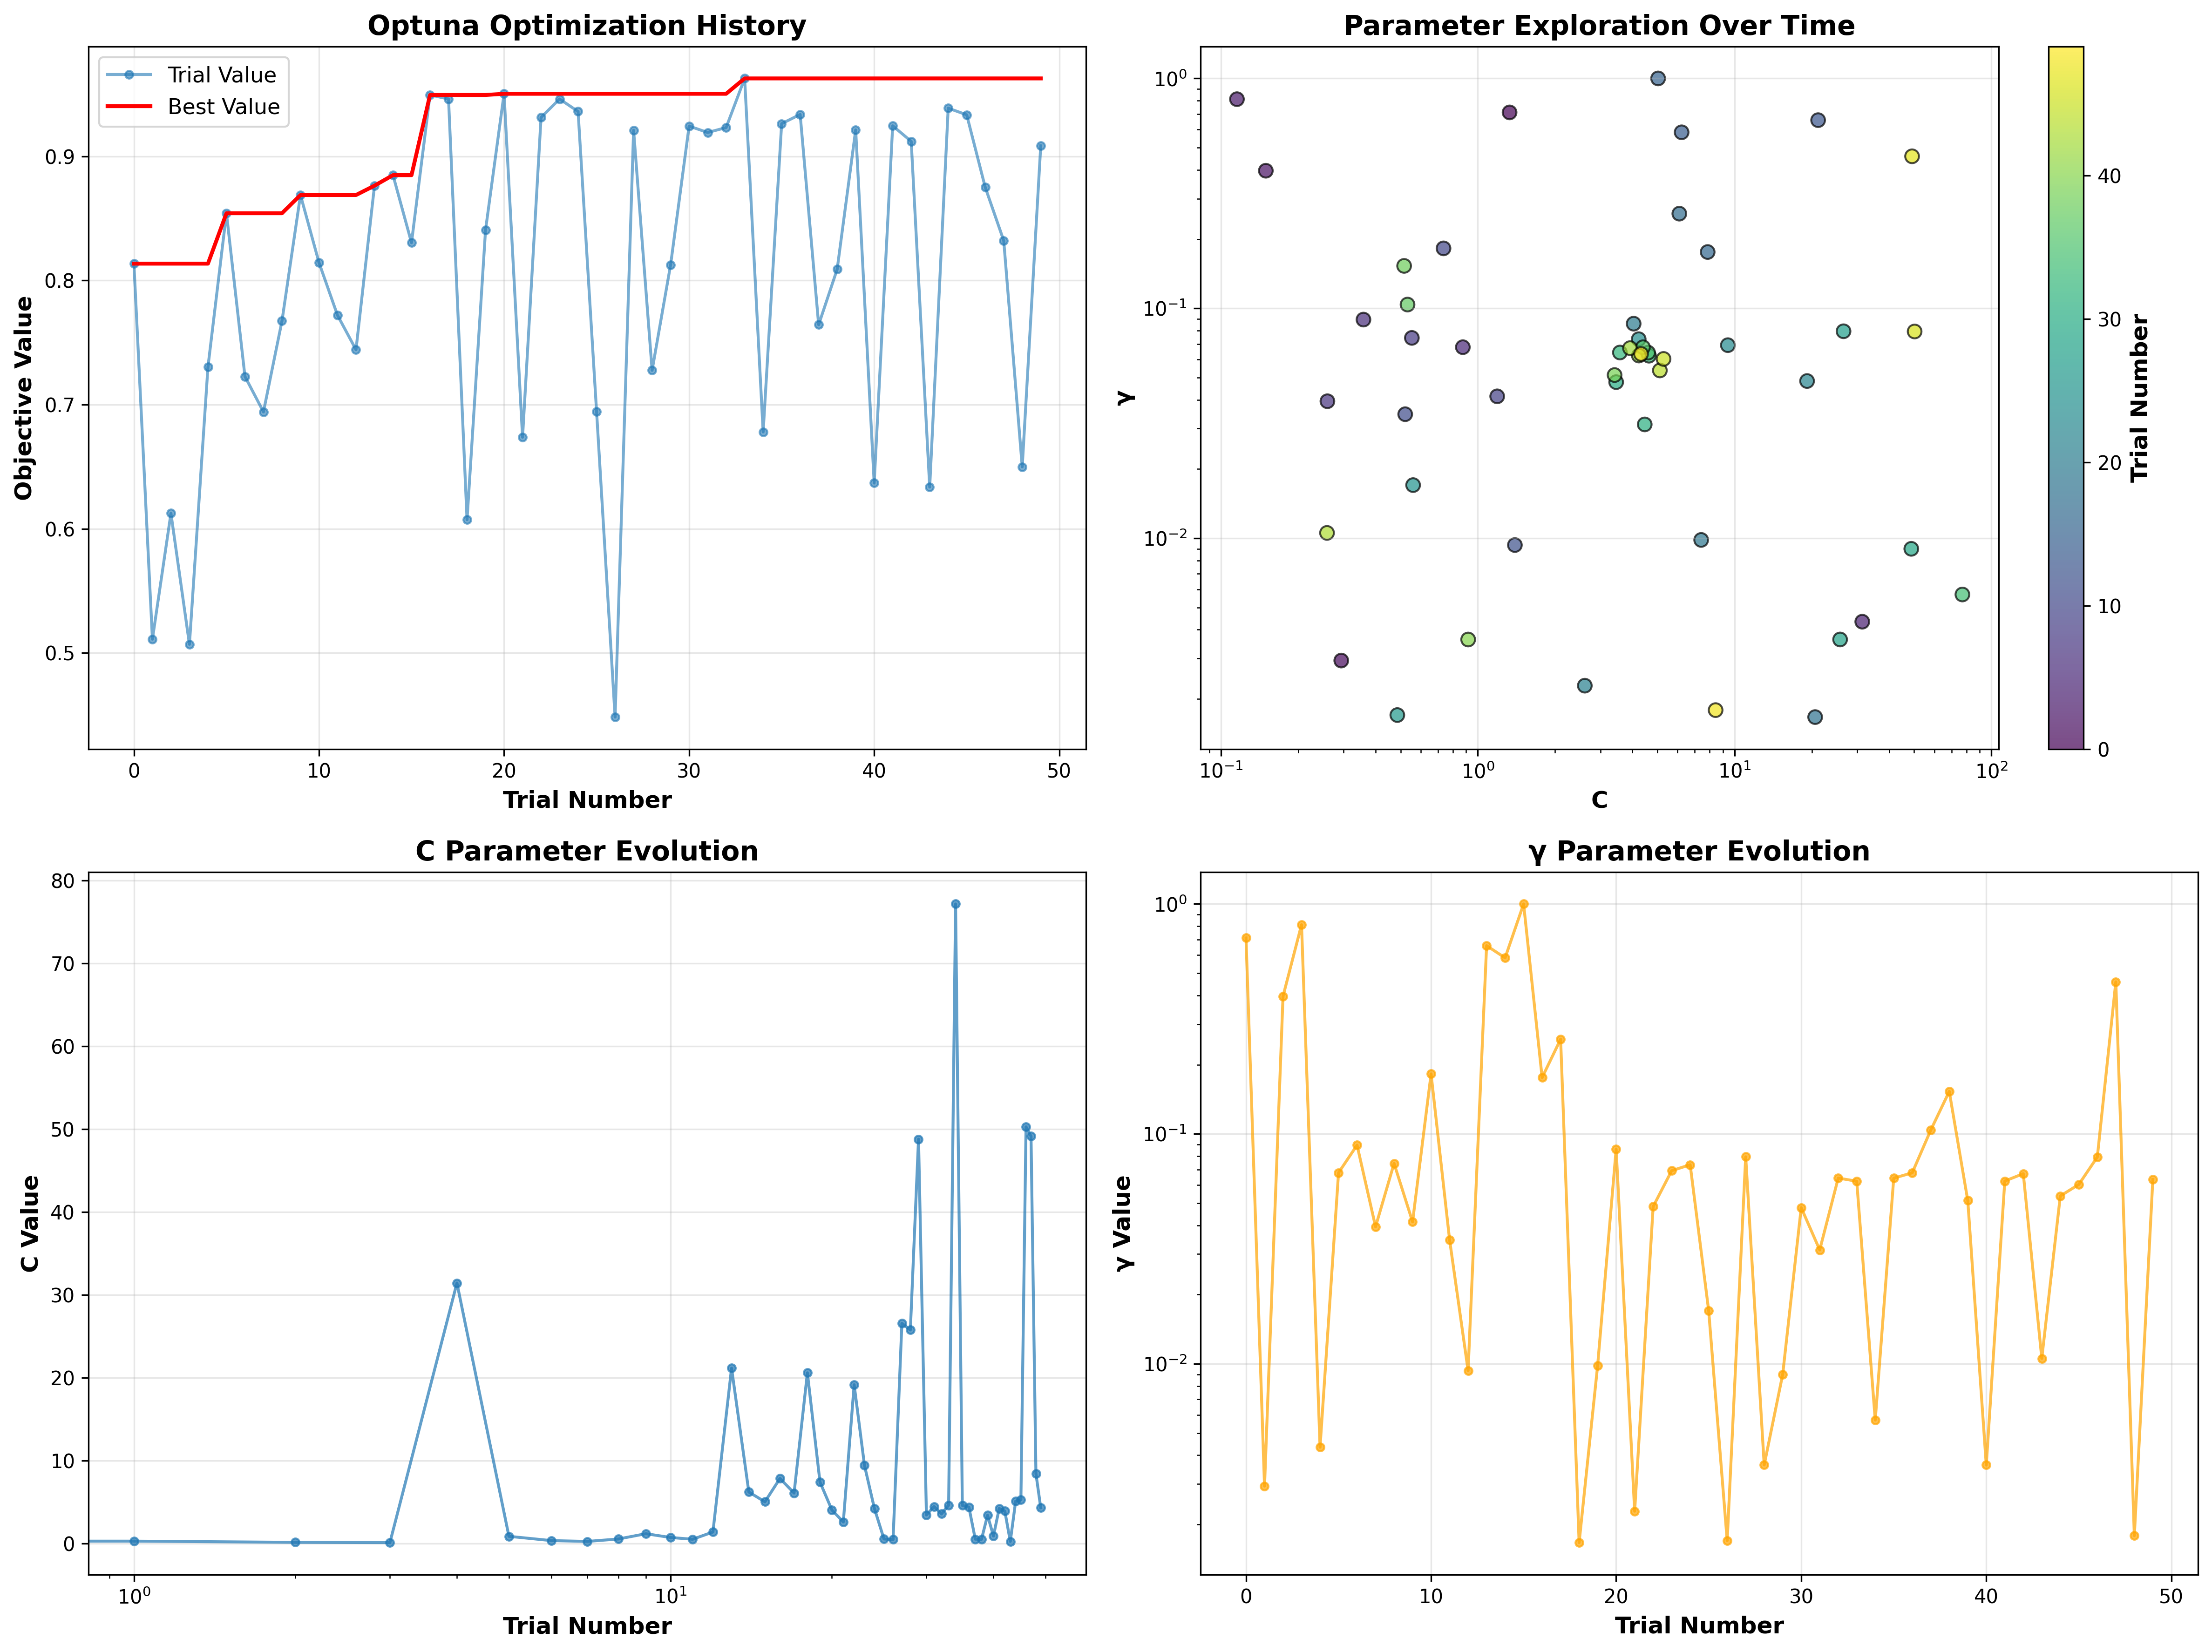
\includegraphics[width=0.9\textwidth]{../figures/optuna_optimization_trace.png}

\vspace{0.3cm}

\begin{alertblock}{Smart Search Strategy}
\textbf{Idea:} Use past evaluations to guide future search, balancing \textcolor{blue}{exploitation} (refine good areas) and \textcolor{red}{exploration} (discover new areas).
\end{alertblock}
\end{frame}

\begin{frame}{Bayesian Optimization: Mathematical Framework}
\textbf{Core Components:}

\begin{columns}[t]
\begin{column}{0.48\textwidth}
\begin{block}{1. Surrogate Model}
Gaussian Process: $f(\lambda) \sim \mathcal{GP}(m(\lambda), k(\lambda, \lambda'))$

\textbf{Predictive distribution:}
\begin{align}
\mu_n(\lambda) &= k_n^T K_n^{-1} \mathbf{y}_n \\
\sigma_n^2(\lambda) &= k(\lambda, \lambda) - k_n^T K_n^{-1} k_n
\end{align}

where:
\begin{itemize}
\item $k_n$: kernel vector at $\lambda$
\item $K_n$: kernel matrix of observed points
\item $\mathbf{y}_n$: observed function values
\end{itemize}
\end{block}
\end{column}

\begin{column}{0.48\textwidth}
\begin{block}{2. Acquisition Function}
\textbf{Expected Improvement (EI):}
\begin{align}
EI(\lambda) &= \mathbb{E}[\max(f^* - f(\lambda), 0)] \\
&= (f^* - \mu(\lambda))\Phi(z) + \sigma(\lambda)\phi(z)
\end{align}

where $z = \frac{f^* - \mu(\lambda)}{\sigma(\lambda)}$, $f^*$ is current best

\textbf{Upper Confidence Bound (UCB):}
$$UCB(\lambda) = \mu(\lambda) + \kappa \sigma(\lambda)$$
\end{block}
\end{column}
\end{columns}

\vspace{0.3cm}

\textbf{Algorithm:}
\begin{enumerate}
\item Initialize with random evaluations
\item Fit GP to observed data $\{(\lambda_i, f(\lambda_i))\}_{i=1}^n$
\item Find $\lambda_{n+1} = \arg\max_\lambda \text{Acquisition}(\lambda)$
\item Evaluate $f(\lambda_{n+1})$ and update data
\item Repeat until budget exhausted
\end{enumerate}
\end{frame}

\begin{frame}{Optuna: Tree-Structured Parzen Estimator (TPE)}
\begin{columns}[t]
\begin{column}{0.55\textwidth}
\textbf{TPE Algorithm:}
\begin{enumerate}
\setlength{\itemsep}{3pt}
\item Split observations by performance quantile $\gamma$:
\begin{itemize}
\item Good: $\mathcal{L} = \{\lambda: f(\lambda) < Q_\gamma\}$
\item Bad: $\mathcal{G} = \{\lambda: f(\lambda) \geq Q_\gamma\}$
\end{itemize}
\item Model densities:
\begin{itemize}
\item $p(\lambda|\mathcal{L})$: density of good configurations
\item $p(\lambda|\mathcal{G})$: density of bad configurations
\end{itemize}
\item Acquisition function:
$$a(\lambda) = \frac{p(\lambda|\mathcal{L})}{p(\lambda|\mathcal{G})}$$
\item Select: $\lambda_{next} = \arg\max_\lambda a(\lambda)$
\end{enumerate}
\end{column}

\begin{column}{0.41\textwidth}
\begin{block}{TPE Advantages}
\begin{itemize}
\setlength{\itemsep}{3pt}
\item \textbf{Efficient}: Lower computational cost than GP
\item \textbf{Flexible}: Handles mixed parameter types
\item \textbf{Scalable}: Works well in high dimensions
\item \textbf{Robust}: Less sensitive to hyperparameters
\end{itemize}
\end{block}

\begin{block}{Optuna Features}
\begin{itemize}
\setlength{\itemsep}{2pt}
\item Pruning: Early stopping of unpromising trials
\item Multi-objective optimization
\item Distributed optimization
\item Integration with ML frameworks
\end{itemize}
\end{block}
\end{column}
\end{columns}

\vspace{0.3cm}

\begin{alertblock}{Key Insight}
TPE focuses sampling on regions where good configurations are dense relative to bad ones.
\end{alertblock}
\end{frame}

\begin{frame}{Hyperparameter Search: Performance Comparison}
\centering
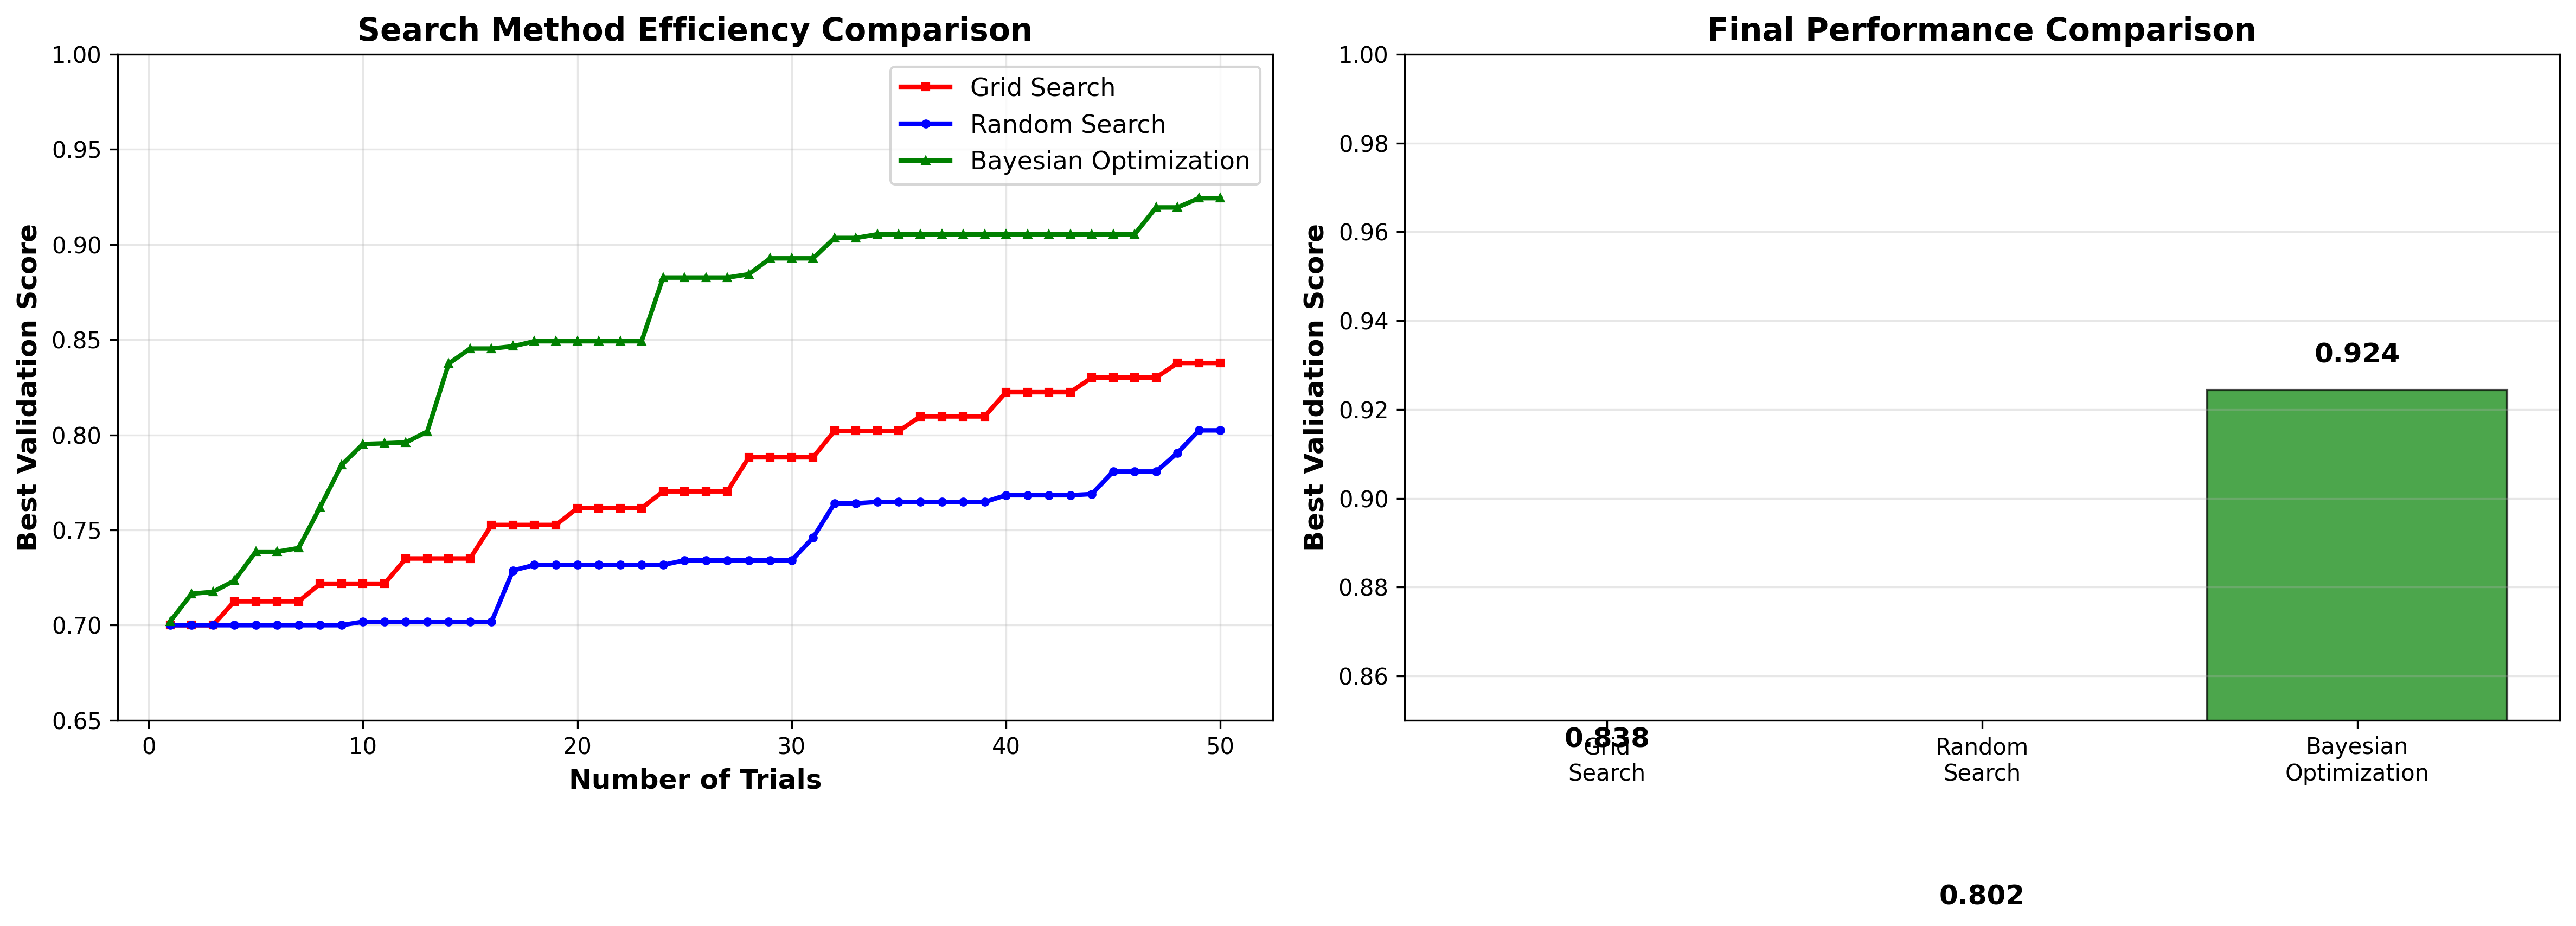
\includegraphics[width=0.9\textwidth]{../figures/search_efficiency_comparison.png}

\vspace{0.3cm}

\begin{columns}[t]
\begin{column}{0.48\textwidth}
\begin{block}{Method Comparison}
\begin{itemize}
\setlength{\itemsep}{3pt}
\item \textbf{Grid Search}: Systematic but inefficient
\item \textbf{Random Search}: Better exploration, good baseline
\item \textbf{Bayesian Optimization}: Fastest convergence, most efficient
\end{itemize}
\end{block}
\end{column}

\begin{column}{0.48\textwidth}
\begin{block}{Recommendations}
\begin{itemize}
\setlength{\itemsep}{3pt}
\item \textbf{Few parameters ($\leq 3$)}: Grid search
\item \textbf{Many parameters ($> 3$)}: Random search
\item \textbf{Expensive evaluations}: Bayesian optimization (Optuna)
\item \textbf{Mixed types}: Optuna TPE
\end{itemize}
\end{block}
\end{column}
\end{columns}

\begin{alertblock}{Best Practice}
Start with random search for quick baseline, then use Bayesian optimization for refinement.
\end{alertblock}
\end{frame}

% ========================================
% Section: Learning Curves
% ========================================

\section{Learning Curves \& Validation Curves}

\begin{frame}{Learning Curves}
\centering
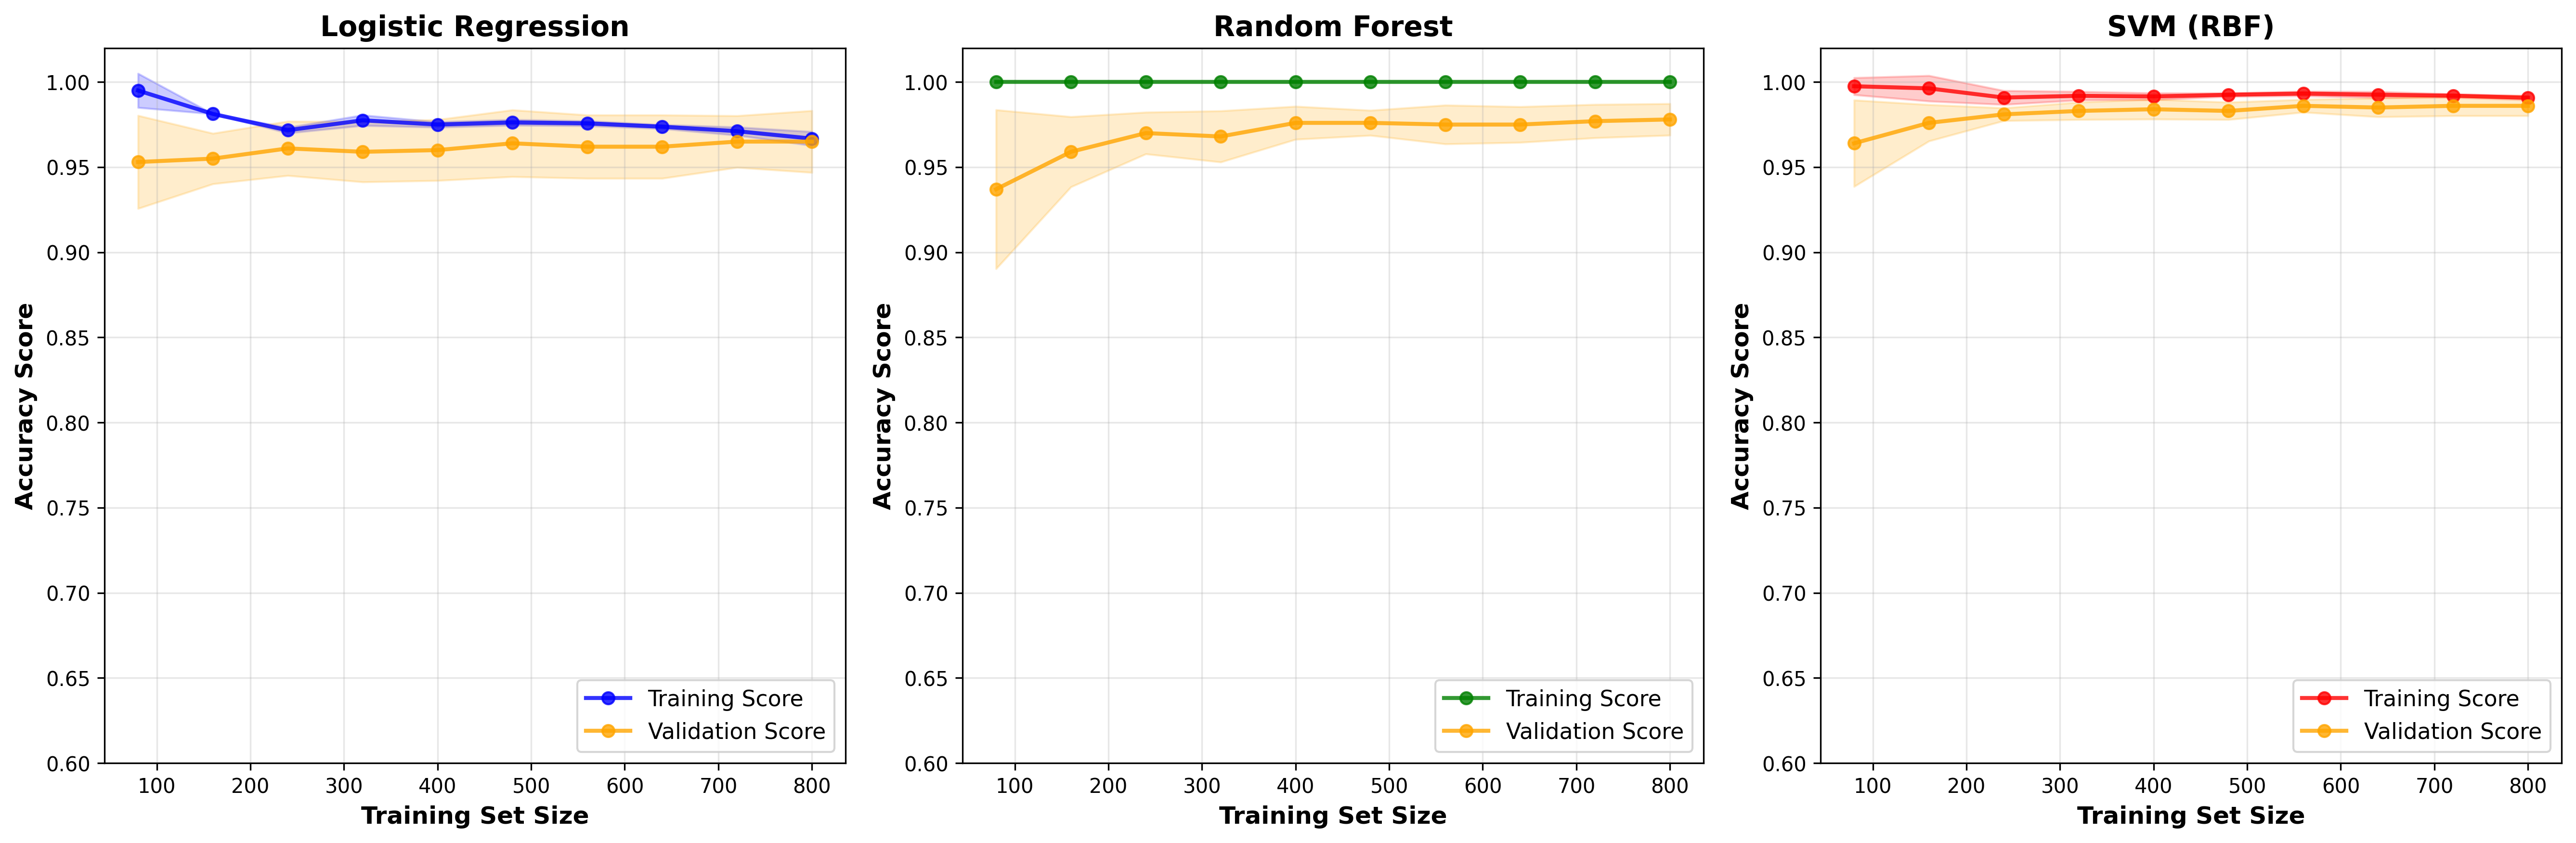
\includegraphics[width=0.9\textwidth]{../figures/learning_curves_cv.png}

\vspace{0.3cm}

\begin{alertblock}{Purpose}
Learning curves help diagnose \textbf{bias} (underfitting) vs \textbf{variance} (overfitting) and determine if more data would help.
\end{alertblock}
\end{frame}

\begin{frame}{Learning Curve Analysis}
\begin{columns}[t]
\begin{column}{0.48\textwidth}
\begin{block}{High Bias (Underfitting)}
\textbf{Symptoms:}
\begin{itemize}
\item Training and validation curves converge
\item Both curves plateau at suboptimal level
\item Large training error
\item Small gap between curves
\end{itemize}

\textbf{Solutions:}
\begin{itemize}
\item Increase model complexity
\item Add more features
\item Reduce regularization
\item Use more flexible model
\end{itemize}
\end{block}
\end{column}

\begin{column}{0.48\textwidth}
\begin{block}{High Variance (Overfitting)}
\textbf{Symptoms:}
\begin{itemize}
\item Large gap between training and validation curves
\item Training error very low
\item Validation error high
\item Curves don't converge
\end{itemize}

\textbf{Solutions:}
\begin{itemize}
\item Get more training data
\item Reduce model complexity
\item Increase regularization
\item Use ensemble methods
\end{itemize}
\end{block}
\end{column}
\end{columns}

\vspace{0.3cm}

\begin{alertblock}{Mathematical Insight}
For a learning algorithm with $m$ training examples:
$$\text{Generalization Error} = \text{Bias}^2 + \text{Variance} + \text{Noise}$$

Learning curves show how this decomposes as $m$ increases.
\end{alertblock}
\end{frame}

\begin{frame}{Validation Curves}
\centering
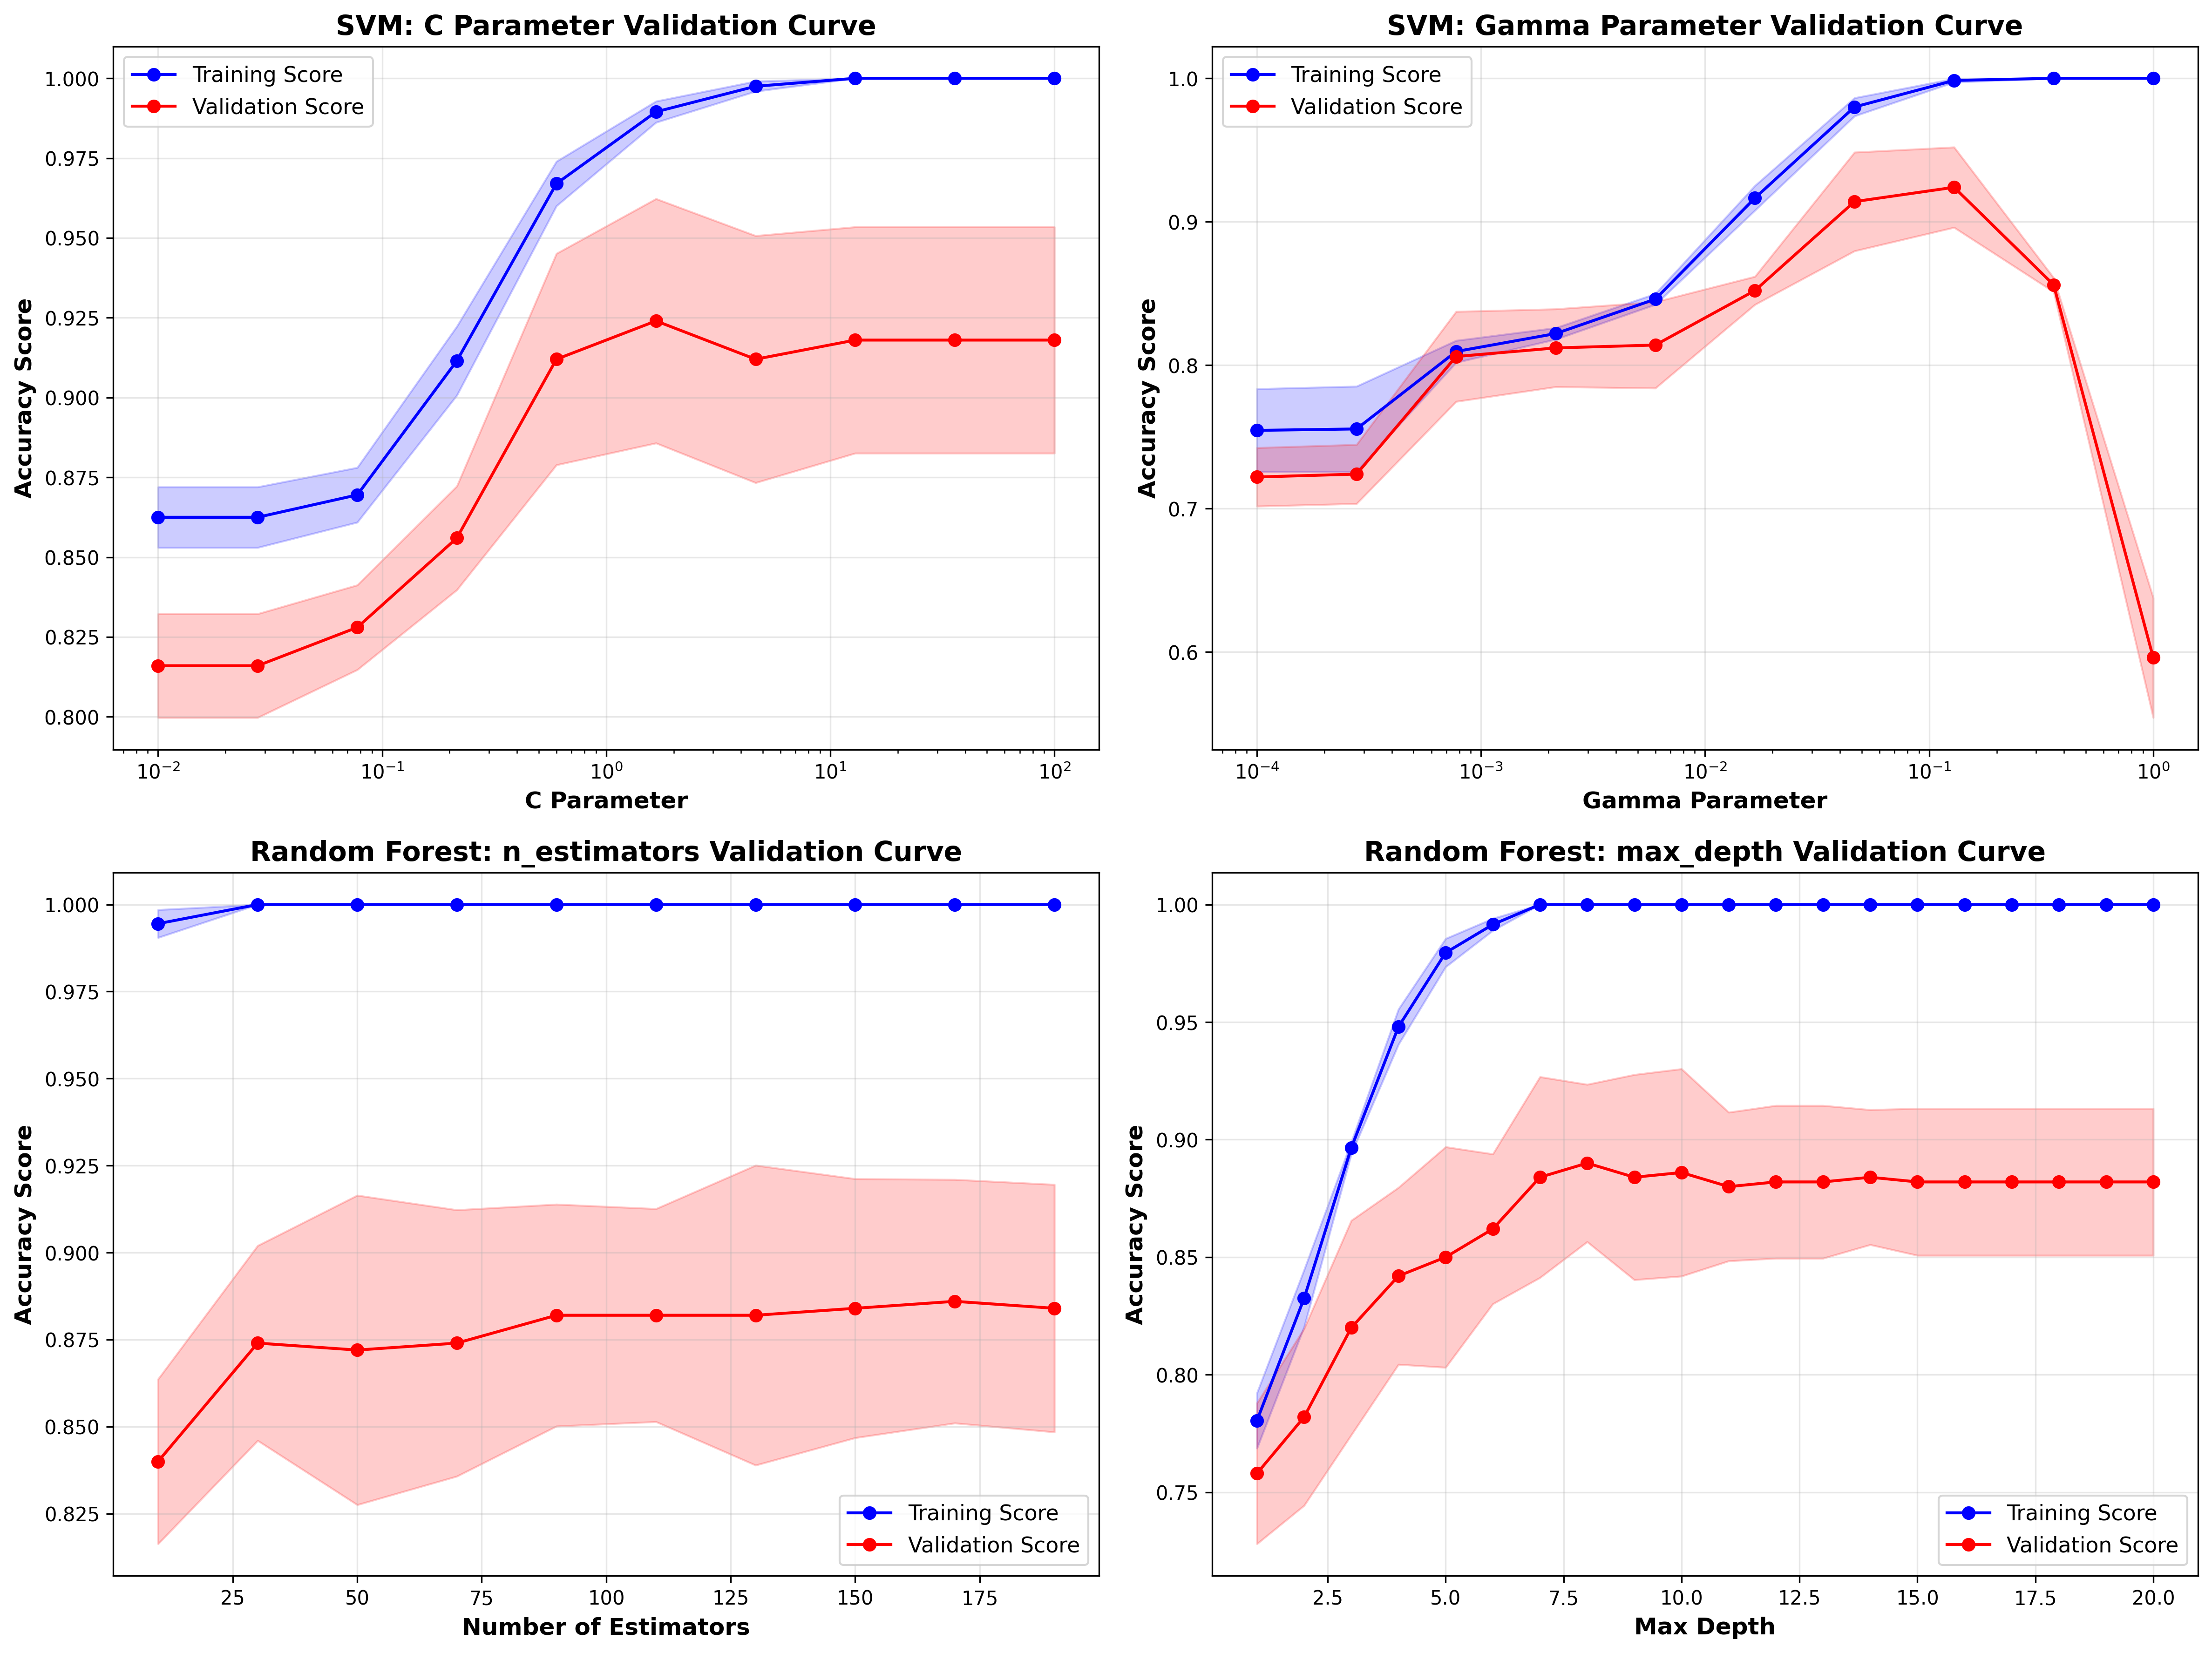
\includegraphics[width=0.9\textwidth]{../figures/validation_curves.png}

\vspace{0.3cm}

\begin{alertblock}{Purpose}
Validation curves show how model performance varies with a single hyperparameter, helping identify optimal values and diagnose overfitting/underfitting.
\end{alertblock}
\end{frame}

\begin{frame}{Interpreting Validation Curves}
\textbf{Typical Pattern Analysis:}

\begin{columns}[t]
\begin{column}{0.48\textwidth}
\begin{block}{Regularization Parameters}
(e.g., SVM C parameter, Ridge $\alpha$)

\textbf{Low values (high regularization):}
\begin{itemize}
\item High bias, low variance
\item Training and validation errors both high
\item Underfitting
\end{itemize}

\textbf{High values (low regularization):}
\begin{itemize}
\item Low bias, high variance
\item Large gap between curves
\item Overfitting
\end{itemize}

\textbf{Optimal region:} Minimum validation error
\end{block}
\end{column}

\begin{column}{0.48\textwidth}
\begin{block}{Model Complexity Parameters}
(e.g., Random Forest depth, SVM $\gamma$)

\textbf{Mathematical relationship:}
$$\text{Complexity} \propto \text{Overfitting Risk}$$

\textbf{Sweet spot identification:}
\begin{enumerate}
\item Find minimum validation error
\item Check if training error is reasonable
\item Ensure curves are not diverging rapidly
\end{enumerate}

\textbf{Cross-validation confidence:}
Error bars show $\pm 1$ standard deviation across CV folds
\end{block}
\end{column}
\end{columns}

\begin{alertblock}{Best Practice}
Always plot both training and validation curves with error bars to make informed hyperparameter choices.
\end{alertblock}
\end{frame}

% ========================================
% Section: Bias-Variance Tradeoff
% ========================================

\section{Bias-Variance Tradeoff}

\begin{frame}{Bias-Variance Decomposition}
\centering
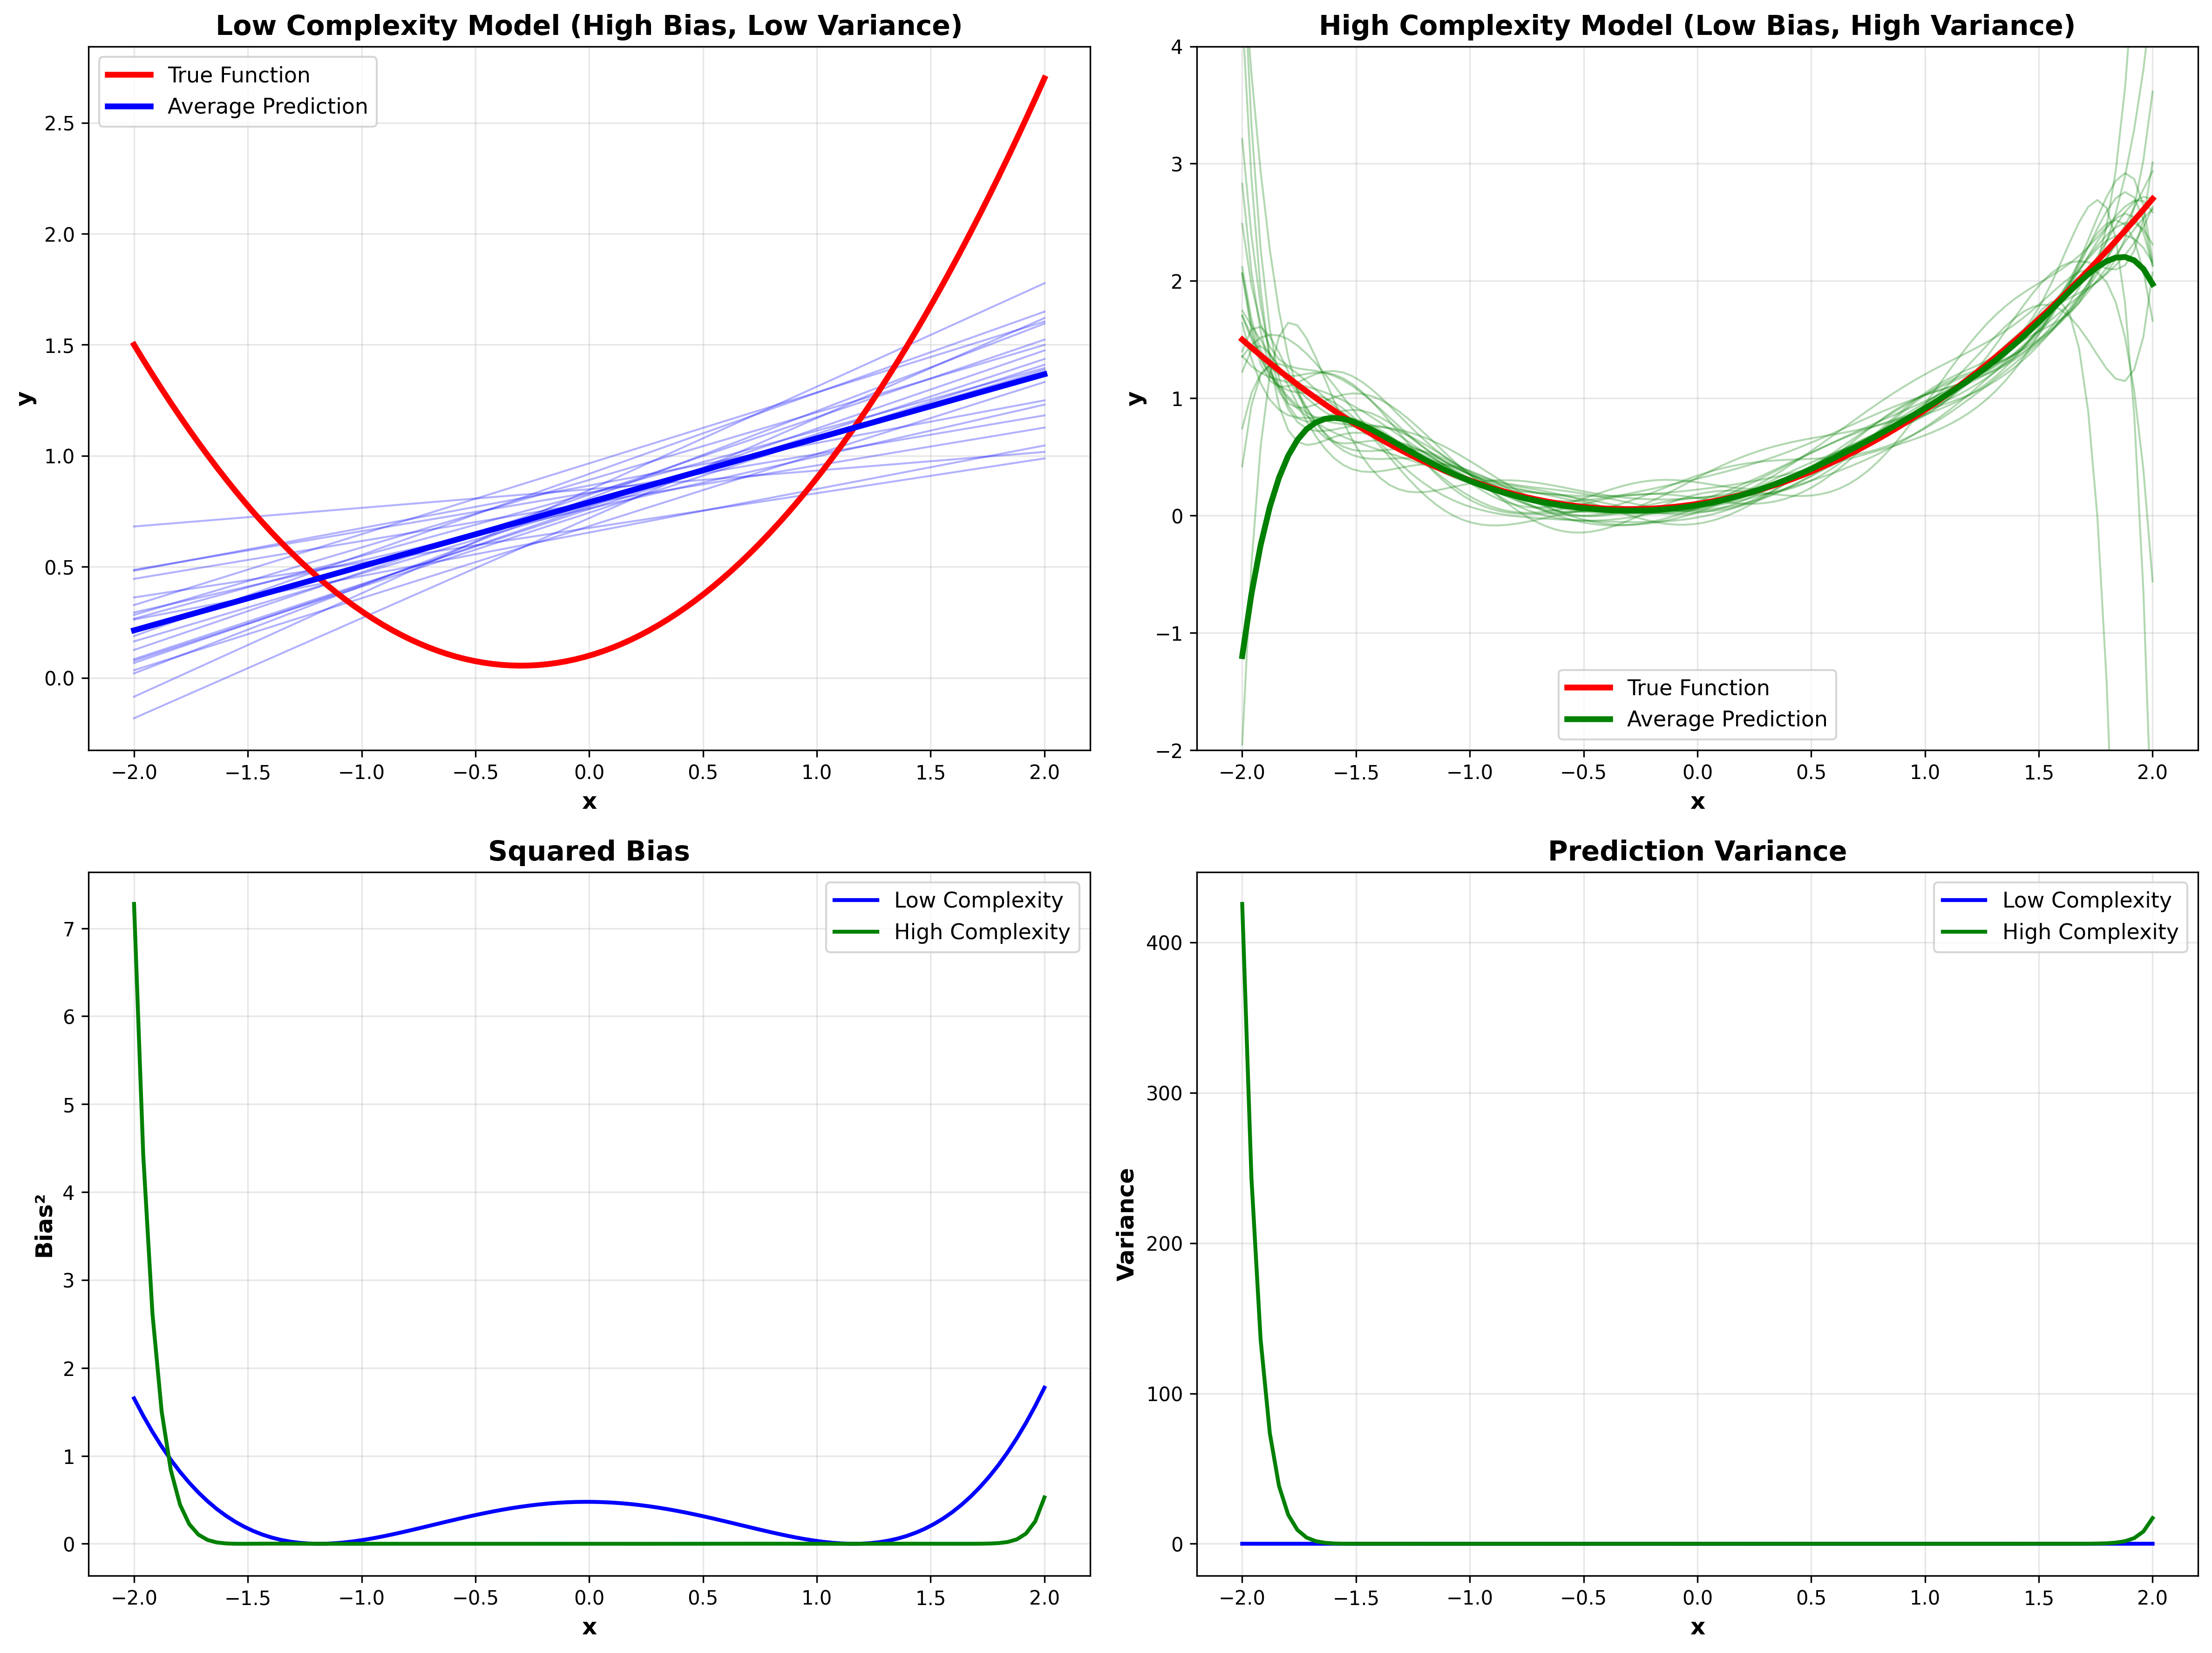
\includegraphics[width=0.9\textwidth]{../figures/bias_variance_tradeoff.png}

\vspace{0.3cm}

\begin{alertblock}{Fundamental Insight}
Cross-validation helps us navigate the bias-variance tradeoff by providing robust estimates of generalization performance across different model complexities.
\end{alertblock}
\end{frame}

\begin{frame}{Bias-Variance Mathematical Framework}
\textbf{Decomposition of Expected Test Error:}

For a target function $f(x)$ and prediction $\hat{f}(x)$:

$$\mathbb{E}[(\hat{f}(x) - f(x))^2] = \text{Bias}^2[\hat{f}(x)] + \text{Var}[\hat{f}(x)] + \sigma^2$$

where:

\begin{align}
\text{Bias}[\hat{f}(x)] &= \mathbb{E}[\hat{f}(x)] - f(x) \\
\text{Var}[\hat{f}(x)] &= \mathbb{E}[(\hat{f}(x) - \mathbb{E}[\hat{f}(x)])^2] \\
\sigma^2 &= \text{Irreducible error (noise)}
\end{align}

\vspace{0.3cm}

\begin{columns}[t]
\begin{column}{0.48\textwidth}
\begin{block}{Cross-Validation \& Bias-Variance}
CV helps estimate:
\begin{itemize}
\item \textbf{Bias}: Through training error analysis
\item \textbf{Variance}: Through CV fold variability
\item \textbf{Optimal complexity}: Bias-variance tradeoff point
\end{itemize}

$$\hat{E}_{CV} \approx \text{Bias}^2 + \text{Var} + \sigma^2$$
\end{block}
\end{column}

\begin{column}{0.48\textwidth}
\begin{block}{Model Selection Strategy}
\begin{enumerate}
\item Compute $\hat{E}_{CV}(\lambda)$ for different complexities
\item Plot learning/validation curves
\item Identify minimum of validation curve
\item Check bias-variance indicators:
\begin{itemize}
\item Training error (bias)
\item CV std deviation (variance)
\end{itemize}
\end{enumerate}
\end{block}
\end{column}
\end{columns}
\end{frame}

% ========================================
% Section: Best Practices
% ========================================

\section{Best Practices \& Guidelines}

\begin{frame}{Cross-Validation Best Practices}
\begin{columns}[t]
\begin{column}{0.48\textwidth}
\begin{block}{Data Splitting}
\begin{itemize}
\setlength{\itemsep}{3pt}
\item \textbf{Stratify} for classification tasks
\item \textbf{Preserve temporal order} for time series
\item \textbf{Group-aware splitting} for clustered data
\item \textbf{Test set isolation}: Never use for model selection
\end{itemize}
\end{block}

\begin{block}{Hyperparameter Search}
\begin{itemize}
\setlength{\itemsep}{3pt}
\item Start with \textbf{random search} for baseline
\item Use \textbf{Bayesian optimization} for expensive evaluations
\item \textbf{Log-uniform sampling} for scale parameters
\item \textbf{Early stopping} for unpromising configurations
\end{itemize}
\end{block}
\end{column}

\begin{column}{0.48\textwidth}
\begin{block}{Statistical Considerations}
\begin{itemize}
\setlength{\itemsep}{3pt}
\item Report \textbf{mean $\pm$ std} of CV scores
\item Use \textbf{paired t-tests} for model comparison
\item Account for \textbf{multiple testing} when comparing many models
\item Consider \textbf{McNemar's test} for classification
\end{itemize}
\end{block}

\begin{block}{Computational Efficiency}
\begin{itemize}
\setlength{\itemsep}{3pt}
\item \textbf{Parallel evaluation} of CV folds
\item \textbf{Caching} of expensive preprocessing steps
\item \textbf{Progressive validation} for large datasets
\item \textbf{Approximate methods} when exact CV is too expensive
\end{itemize}
\end{block}
\end{column}
\end{columns}

\begin{alertblock}{Golden Rule}
\textbf{Never} use the test set for any decision making during model development. Reserve it solely for final performance evaluation.
\end{alertblock}
\end{frame}

\begin{frame}{Common Pitfalls \& How to Avoid Them}
\begin{columns}[t]
\begin{column}{0.48\textwidth}
\begin{block}{Data Leakage}
\textbf{Problem:} Information from validation/test leaks into training

\textbf{Examples:}
\begin{itemize}
\item Scaling on entire dataset before splitting
\item Feature selection using all data
\item Temporal leakage in time series
\end{itemize}

\textbf{Solution:} Apply preprocessing within each CV fold
\end{block}

\begin{block}{Look-ahead Bias}
\textbf{Problem:} Using future information for prediction

\textbf{Example:} Standard CV on time series data

\textbf{Solution:} Time series CV with forward chaining
\end{block}
\end{column}

\begin{column}{0.48\textwidth}
\begin{block}{Selection Bias}
\textbf{Problem:} Multiple testing without correction

\textbf{Example:} Comparing 100 models, reporting best CV score

\textbf{Solution:} Bonferroni correction or separate validation set for selection
\end{block}

\begin{block}{Inappropriate CV Method}
\textbf{Problems:}
\begin{itemize}
\item LOOCV with large datasets (unstable)
\item Standard CV with imbalanced data
\item Ignoring data structure (groups, time)
\end{itemize}

\textbf{Solution:} Choose CV method based on data characteristics
\end{block}
\end{column}
\end{columns}

\begin{alertblock}{Validation}
Always ask: \textit{"Does my validation procedure realistically simulate deployment conditions?"}
\end{alertblock}
\end{frame}

\begin{frame}{Hyperparameter Search Space}
\centering
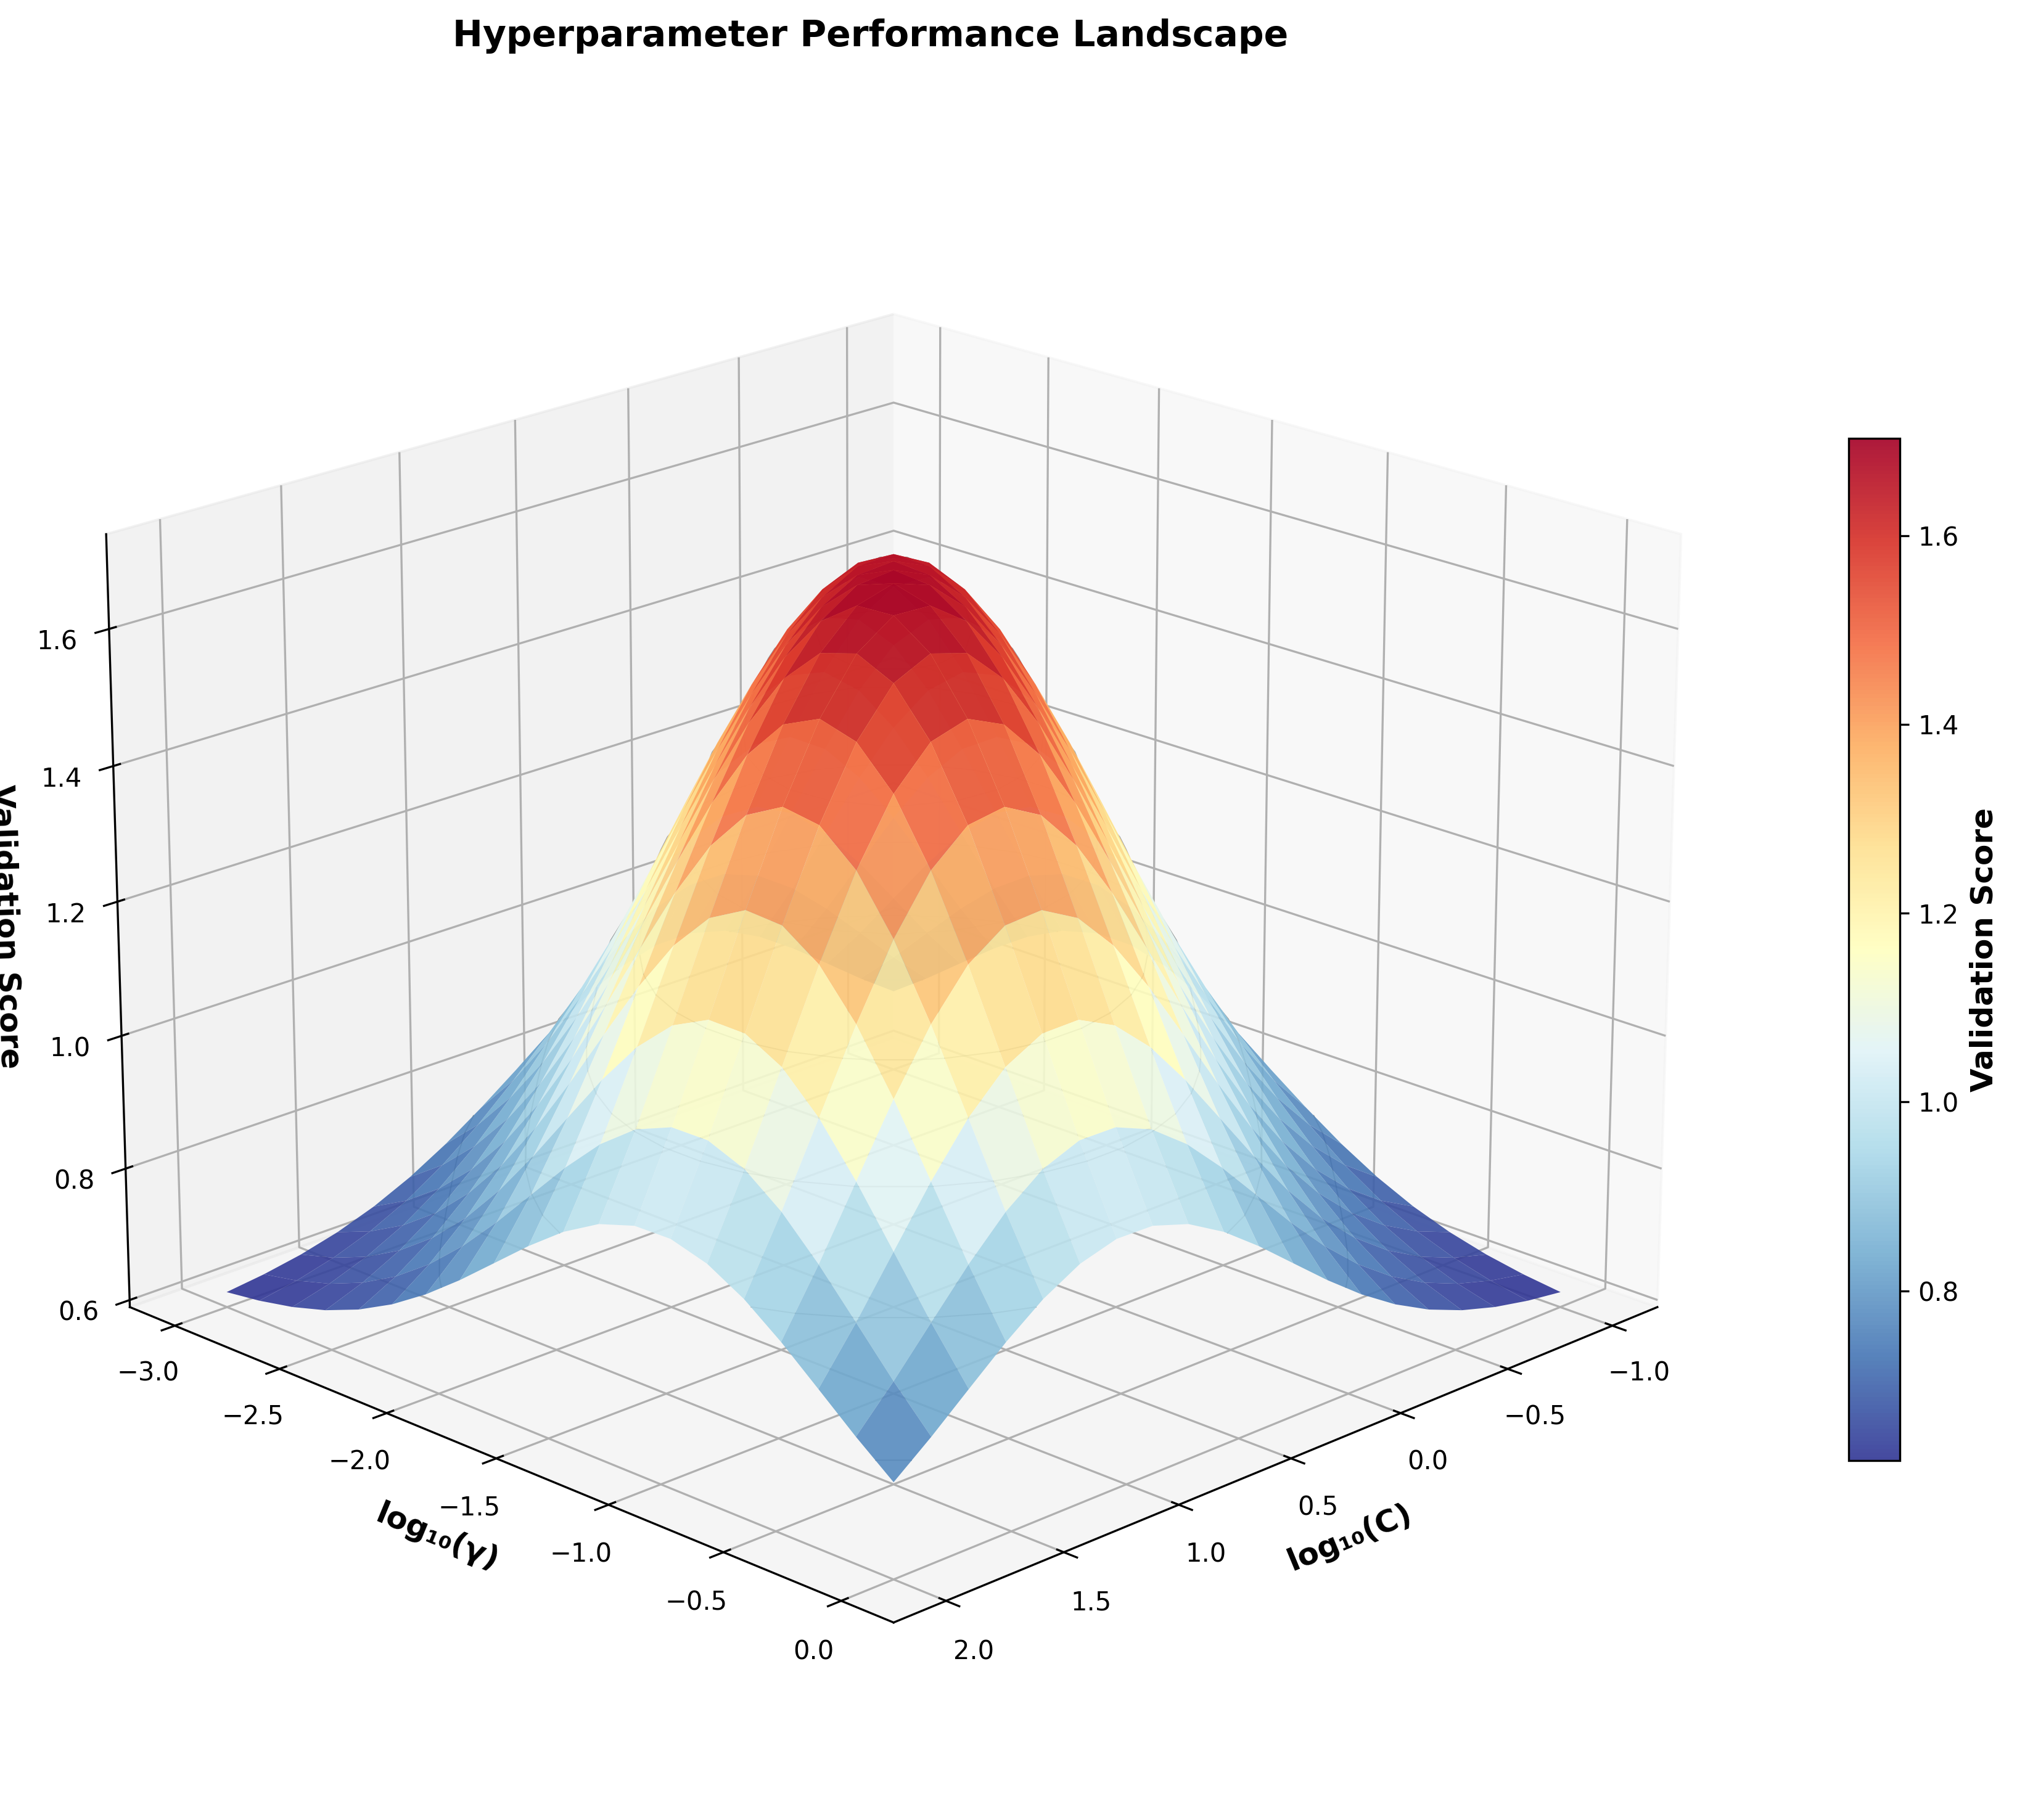
\includegraphics[width=0.8\textwidth]{../figures/hyperparameter_surface.png}

\vspace{0.3cm}

\begin{alertblock}{Key Insight}
Hyperparameter optimization landscapes are often complex with multiple local optima, making smart search strategies essential for finding good solutions efficiently.
\end{alertblock}
\end{frame}

% ========================================
% Section: Summary
% ========================================

\section{Summary}

\begin{frame}{Summary: Model Validation Hierarchy}
\vspace{0.3cm}

\textbf{Model Validation Hierarchy:}

\begin{center}
\begin{tabular}{c}
\textcolor{green!80!black}{\textbf{Original Dataset}} \\
$\downarrow$ \\
\textcolor{yellow!80!black}{\textbf{Train / Validation / Test Split}} \\
$\downarrow$ \quad $\downarrow$ \quad $\downarrow$ \\
\begin{tabular}{@{}c@{\hspace{1cm}}c@{\hspace{1cm}}c@{}}
\textcolor{blue!80!black}{\textbf{Training Set}} & \textcolor{orange!80!black}{\textbf{Validation Set}} & \textcolor{red!80!black}{\textbf{Test Set}} \\
\textcolor{blue!80!black}{(60-80\%)} & \textcolor{orange!80!black}{(10-20\%)} & \textcolor{red!80!black}{(10-20\%)} \\
$\downarrow$ & $\downarrow$ & $\downarrow$ \\
\textcolor{purple!80!black}{\textbf{Cross-Validation}} & \textcolor{cyan!80!black}{\textbf{Hyperparameter}} & \textcolor{pink!80!black}{\textbf{Final}} \\
\textcolor{purple!80!black}{(Model Selection)} & \textcolor{cyan!80!black}{Tuning} & \textcolor{pink!80!black}{Evaluation}
\end{tabular}
\end{tabular}
\end{center}

\vspace{0.3cm}

\begin{alertblock}{Best Practice Workflow}
\begin{enumerate}
\item Split data
\item Use CV for model selection
\item Tune hyperparameters on validation set
\item Final evaluation on test set (once!)
\end{enumerate}
\end{alertblock}
\end{frame}

\begin{frame}{Key Takeaways}
\begin{columns}[t]
\begin{column}{0.48\textwidth}
\begin{block}{Validation Methods}
\begin{itemize}
\setlength{\itemsep}{3pt}
\item \textbf{Holdout}: Fast but high variance
\item \textbf{K-fold CV}: Best general-purpose method
\item \textbf{LOOCV}: Unbiased but expensive
\item \textbf{Stratified}: Essential for imbalanced data
\item \textbf{Time series CV}: Preserves temporal order
\end{itemize}
\end{block}

\begin{block}{Method Selection Guide}
\begin{itemize}
\setlength{\itemsep}{2pt}
\item Small data (n < 1000): 10-fold CV or LOOCV
\item Large data (n > 10000): 5-fold CV or holdout
\item Imbalanced: Stratified k-fold
\item Time series: Forward chaining
\item Grouped data: Group k-fold
\end{itemize}
\end{block}
\end{column}

\begin{column}{0.48\textwidth}
\begin{block}{Hyperparameter Search}
\begin{itemize}
\setlength{\itemsep}{3pt}
\item \textbf{Grid search}: $\leq$3 parameters, comprehensive
\item \textbf{Random search}: >3 parameters, efficient baseline
\item \textbf{Bayesian optimization}: Expensive evaluations, smart search
\item \textbf{Use proper distributions}: Log-uniform for scale parameters
\end{itemize}
\end{block}

\begin{block}{Critical Principles}
\begin{itemize}
\setlength{\itemsep}{2pt}
\item Never use test set for model selection
\item Avoid data leakage at all costs
\item Report confidence intervals (mean ± std)
\item Match validation to deployment conditions
\item Use learning curves to diagnose bias/variance
\end{itemize}
\end{block}
\end{column}
\end{columns}

\begin{alertblock}{Remember}
\textbf{Cross-validation is not just about getting a number—it's about making principled decisions about model selection, hyperparameter tuning, and understanding model behavior.}
\end{alertblock}
\end{frame}

\begin{frame}[standout]
Questions?
\end{frame}

\end{document}